\chapter{Generative models for fast particle-cloud simulations}
\label{sec:04_models}

\section{Message passing GANs}
\label{sec:04_mpgan}

In this chapter we describe two novel generative models for fast simulations of particle clouds in HEP.
We first introduce the message-passing generative adversarial network (MPGAN) trained on high-energy \jetnet jets.
To our knowledge, it was the first generative model in HEP to effectively simulate point cloud data, and represented a breakthrough in the performance of ML-based fast simulations, leveraging sparse and efficient representations naturally suited to our data.
It builds on top of the success of graph neural networks (GNNs) in learning from point clouds in computer vision, but is designed to take advantage of additional key inductive biases in HEP data, such as the non-local correlations between particles in a jet and their varying cardinalities.

The landscape of point cloud generative models in HEP and computer vision at the time of MPGAN's publication was detailed in Chapter~\ref{sec:04_mpgan_genhep}.
In this section, we first discuss evaluation metrics used to compare MPGAN to existing models (Section~\ref{sec:04_mpgan_geneval}) before describing the model architecture (Section~\ref{sec:04_mpgan_arch}).
We then discuss experimental results, first on MNIST handwritten digits as a testbench in Section~\ref{sec:04_mpgan_mnist}, and finally on the \jetnet dataset in Section~\ref{sec:04_mpgan_exp}.


\subsection{Evaluation}
\label{sec:04_mpgan_geneval}

Evaluating generative models is a difficult task; however, there has been extensive work in this area in both the physics and computer-vision communities.
We provide here a brief overview of the metrics used for comparing MPGAN and the baseline models discussed above, leaving a more detailed discussion, as well as an introduction to the novel metrics we develop for this task, to Chapter~\ref{sec:04_evaluating}.

\subsubsection{Physics-inspired metrics}

An accurate jet simulation algorithm should reproduce both low-level and high-level features (such as those described in Chapter~\ref{sec:04_mpgan_genhep}); hence, a standard method of validating generative models, which we too employ, is to compare the distributions of such features between the real and generated samples~\cite{deOliveira:2017pjk, Paganini:2017dwg, ATL-SOFT-PUB-2020-006, Erdmann:2018jxd, Carminati:2020kym, Sekmen:2016iql}. 

For application in HEP, a generative model needs to produce jets with physical features indistinguishable from real.
Therefore, we propose the validation criteria that differences between real and generated sample features may not exceed those between sets of randomly chosen real samples.
To verify this, we use bootstrapping to compare between random samples of only real jets as a baseline. 

A practically useful set of features to validate against are the so-called ``energy-flow polynomials'' (EFPs)~\cite{Komiske:2017aww}, which are a type of multi-particle correlation functions. 
Importantly, the set of all EFPs forms a linear basis for all experimentally useful --- i.e., all infrared- and colinear- (IRC-) safe --- jet-level features / observables.
Therefore, we claim that if we observe all EFP distributions to be reproduced with high fidelity and to match the above criteria, we can conclude with strong confidence that our model is outputting accurate particle clouds. 

\subsubsection{Computer-vision-inspired metrics}
A popular metric for evaluating images which has been shown to be sensitive to output quality and mode-collapse --- though it has its limitations~\cite{borji2021} --- is the Fr\'{e}chet Inception Distance~\cite{TTUR} (FID). 
FID is defined as the Fr\'{e}chet distance between Gaussian distributions fitted to the activations of a fully-connected layer of the Inception-v3 image classifier in response to real and generated samples. 
We develop a particle-cloud-analogue of this metric, which we call Fr\'{e}chet ParticleNet Distance (FPND), using the state-of-the-art (SOTA) ParticleNet graph convolutional jet classifier~\cite{Qu:2019gqs} in lieu of the Inception network.
We note that FPND and comparing distributions as above are conceptually equivalent, except here instead of physically meaningful and easily interpretable features, we are comparing those found to be statistically optimum for distinguishing jets.

Two common metrics for evaluating point cloud generators are coverage (COV) and minimum matching distance (MMD)~\cite{rgan}. 
Both involve finding the closest point cloud in a sample $X$ to each cloud in another sample $Y$, based on a metric such as the Chamfer distance or the earth mover's distance. 
Coverage is defined as the fraction of samples in $X$ which were matched to one in $Y$, measuring thus the diversity of the samples in $Y$ relative to $X$, and MMD is the average distance between matched samples, measuring the quality of samples. 
We use both, and due to drawbacks of the Chamfer distance pointed out in Ref.~\cite{rgan}, for our distance metric choose only the analogue of the earth mover's distance for particle clouds a.k.a. the energy mover's distance (EMD)~\cite{Komiske:2019fks}. 
We discuss the effectiveness and complementarity of all four metrics in evaluating clouds in Section~\ref{sec:04_mpgan_results}.


\subsection{Architecture}
\label{sec:04_mpgan_arch}

We describe now the architecture of the MPGAN model (Figure~\ref{fig:04_mpgan_arch}), noting particle-cloud-motivated aspects compared to its r-GAN and GraphCNN-GAN predecessors (see Chapter~\ref{sec:04_mpgan_genhep}).

\begin{figure}[t!]
    \centering
    \centerline{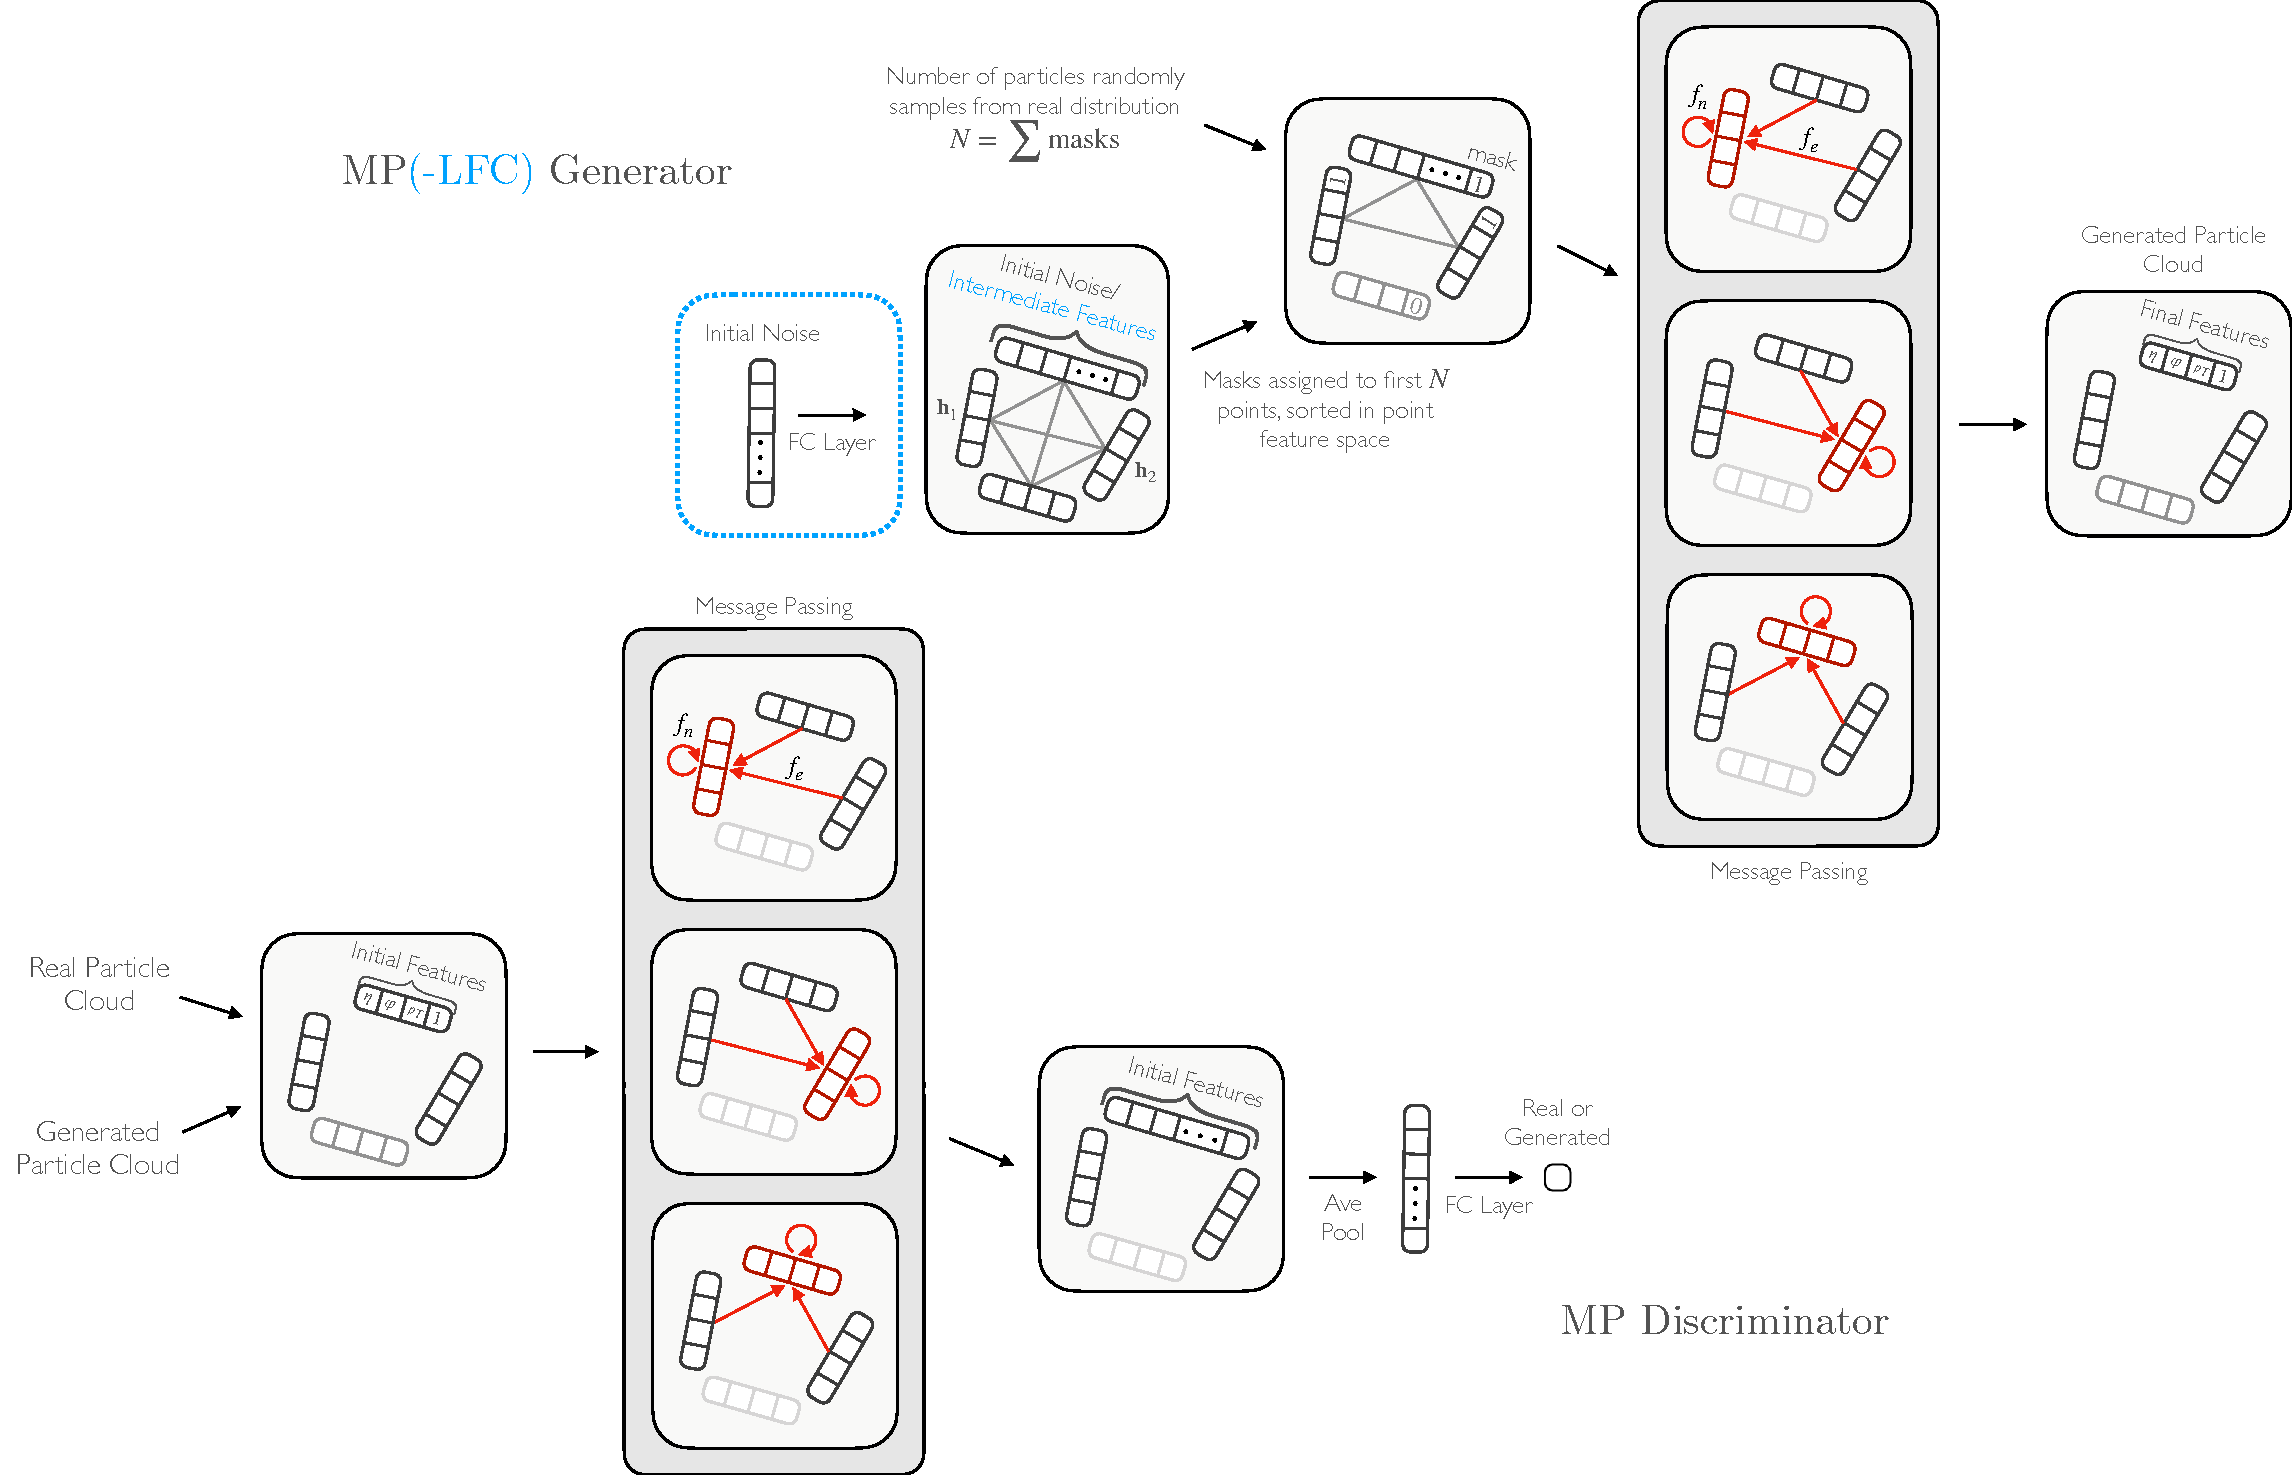
\includegraphics[width=\textwidth]{figures/04-ML4Sim/mpgan/mparch_wide.pdf}}
    \caption[Top: The MP generator uses message passing to generate a particle cloud.]{Top: The MP generator uses message passing to generate a particle cloud. 
    In blue is the initial latent vector and FC layer part of the MP-LFC variant.
    Bottom: The MP discriminator uses message passing to classify an input particle cloud as real or generated.}
    \label{fig:04_mpgan_arch}
\end{figure}

\subsubsection{Message passing}

Jets originate from the decay and hadronization of a single source-particle; hence, they end up with important high-level jet features and a rich global structure, known as the jet substructure~\cite{larkoski2020jet}, stemming from the input particle. 
Indeed, any high-level feature useful for analyzing jets, such as jet mass or multi-particle correlations, is necessarily global~\cite{Komiske:2017aww}.  
Because of this, while past work in learning on point clouds~\cite{dynamicgraphcnn, monti2017geometric, Qu:2019gqs}, including GraphCNN-GAN, has used a locally connected graph structure and convolutions for message passing, we choose a fully connected graph, equally weighting messages from all particles in the clouds. 
Rather than subtracting particle features for messages between particles, useful in graph convolutions to capture local differences within a neighborhood, the respective features are concatenated to preserve the global structure (the difference between particle features is also only physically meaningful if they are in the 4-vector representation of the Lorentz group). 
During the update step in the message passing we find it empirically beneficial to incorporate a residual connection to previous particle features.

The operation can be described as follows. 
For an $N$-particle cloud $J^t = \{p_1^t, \cdots, p_N^t\}$ after $t$ iterations of message passing, with $t=0$ corresponding to the original input cloud, each particle $p^t_i$ is represented by features $\cvec{h}^t_i$.
One iteration of message passing is then defined as
\begin{align}
        \label{eqn:mpm} \cvec{m}^{t+1}_{ij} &= f_e^{t+1}(\cvec{h}^t_i \oplus \cvec{h}^t_j), \\
        \label{eqn:mph} \cvec{h}^{t+1}_i &= f_n^{t+1}(\cvec{h}^t_i \oplus \sum_{j \in J} \cvec{m}^{t+1}_{ij})\,,
\end{align}
where $\cvec{m}^{t+1}_{ij}$ is the message vector sent from particle $j$ to particle $i$, $\cvec{h}^{t+1}_i$ are the updated features of particle $i$, and $f_e^{t+1}$ and $f_n^{t+1}$ are arbitrary functions which, in our case, are implemented as multilayer perceptrons (MLPs) with 3 FC layers.
% Ablation studies using our message passing operation but with locally connected topologies are discussed in App.~\ref{app:04_mpgan_locallyconnected}.


\subsubsection{Generator}

We test two initializations of a particle cloud for the MPGAN generator: (1) directly initializing the cloud with $N$ particles, each with $L$ randomly sampled features, which we refer to as the MP generator, and (2) inputting a single $Z$-dimensional latent noise vector and transforming it via an FC layer into an $N\times L$-dimensional matrix, which we refer to as the MP-Latent-FC (MP-LFC) generator. 
MP-LFC uses a latent space which can intuitively be understood as representing the initial source particle's features along with parameters to capture the stochasticity of the jet production process.
Due to the complex nature of this process, however, we posit that this global, flattened latent space cannot capture the full phase space of individual particle features. 
Hence, we introduce the MP generator, which samples noise directly per particle, and find that it outperforms MP-LFC (Table~\ref{tab:04_mpgan_results}).

\subsubsection{Discriminator}

We find the MP generator, in conjunction with a PointNet discriminator, to be a significant improvement on every metric compared to FC and GraphCNN generators.
However, the jet-level features are not yet reproduced to a high enough accuracy (Section~\ref{sec:04_mpgan_results}).
While PointNet is able to capture global structural information, it can miss the complex interparticle correlations in real particle clouds.
We find we can overcome this limitation by incorporating message passing in the discriminator as well as in the generator.
Concretely, our MP discriminator receives the real or generated cloud and applies MP layers to produce intermediate features for each particle, which are then aggregated via a feature-wise average-pooling operation and passed through an FC layer to output the final scalar feature.
We choose 2 MP layers for both networks. 

\subsubsection{Variable-sized clouds}

In order to handle clouds with varying numbers of particles, as typical of jets, we introduce an additional binary ``masking'' particle feature classifying the particle as genuine or zero-padded. 
Particles in the zero-padded class are ignored entirely in the message passing and pooling operations. 
The MP generator adds mask features to the initial particle cloud, using an additional input of the size of the jet $N$, sampled from the real distribution per jet type, before the message passing layers, based on sorting in particle feature space. 
Ablation studies with alternative (as well as without) masking strategies are discussed in App.~\ref{app:04_mpgan_masking}.

\subsection{Experiments on MNIST handwritten digits}
\label{sec:04_mpgan_mnist}

Before applying MPGAN to the \jetnet dataset, we test it initially on point-cloud versions of the MNIST handwritten digits dataset~\cite{deng2012mnist}.
Practically, these were highly useful during the development of the model, while exploring architectures, hyperparameters, and training strategies, as they provided a simpler test-bench as well as an easy way to visually evaluate the model.

We consider two MNIST datasets.
First, a sparse graph representation of the MNIST dataset, where from each image we select the 100 highest intensity pixels as the nodes of a fully connected graph, with their feature vectors consisting of the $x$, $y$ coordinates and intensities. 
This is directly analogous to selecting the coordinates and momenta of the highest momentum particles in a jet or highest energy hits in a detector.
The second dataset, known as the MNIST superpixels dataset~\cite{monti2017geometric}, was created by converting each MNIST image into 75 superpixels, corresponding to the nodes of a graph. 
The centers and intensities of the superpixels comprise the hidden features of the nodes.
% Edge features for both datasets are chosen to be the Euclidean distance between the connected nodes. 

We train MPGAN separately for each digit, analogous to independent trainings for different jet classes.
The best parameters per-digit are chosen using a variation of FID adopted for point clouds, using the hidden features of the MoNet classifier~\cite{monti2017geometric}.
The comparison between the real and MPGAN-generated samples for both datasets can be seen in Figure~\ref{fig:04_mpgan_mnist}.
We observe that the model is able to reproduce the real samples with high fidelity and little evidence of mode dropping.

\begin{figure}[ht]
    \centering
    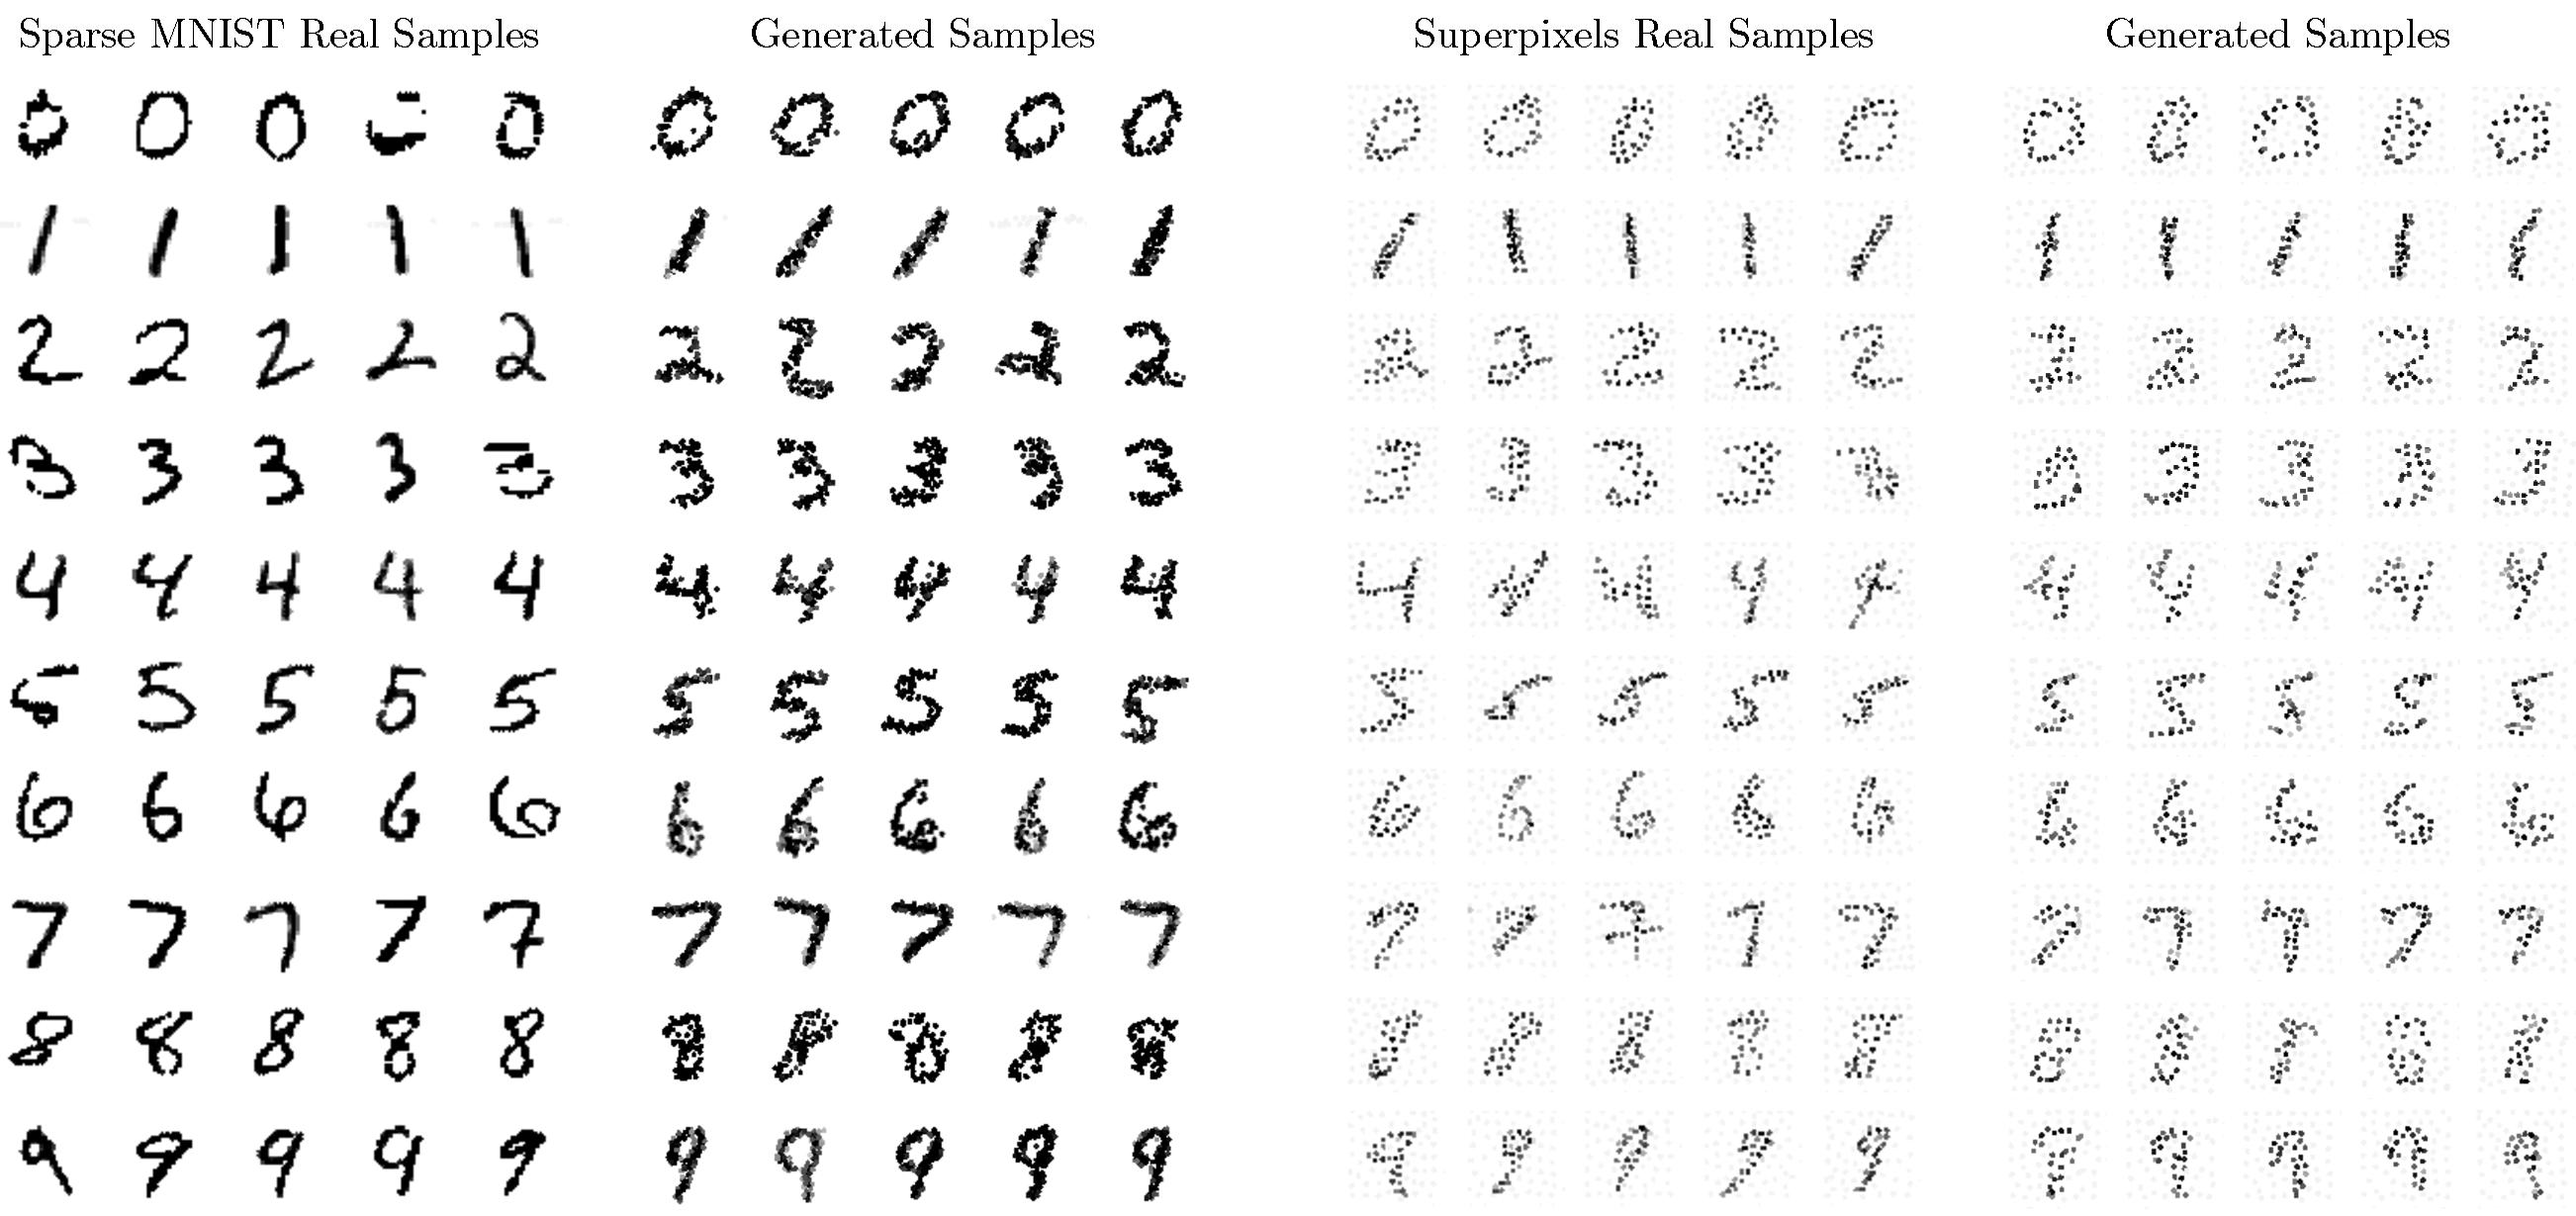
\includegraphics[width=\textwidth]{figures/04-ML4Sim/mpgan/real_gen.pdf}
    \caption{Samples from our sparse MNIST dataset (far left) compared to samples from MPGAN (center left). 
    Samples from the MNIST superpixels dataset (center right) compared to samples from MPGAN (far right).\label{fig:04_mpgan_mnist}}
\end{figure}


\subsection{Experiments on jets}
\label{sec:04_mpgan_exp}

We now present results on the \jetnet dataset.
We first discuss the evaluation metrics, then the results of the MPGAN model compared to several baseline point-cloud generative models, as well as extensive discussion on both the architecture and evaluation metric choices.

\subsubsection{Evaluation}
\label{sec:04_mpgan_eval}

We use four techniques discussed in Section~\ref{sec:04_mpgan_geneval} for evaluating and comparing models. 
Distributions of physical particle and jet features are compared visually and quantitatively using the Wasserstein-1 (\wass) distance between them. 
For ease of evaluation, we report (1) the average scores of the three particle features (\wassp) $\etarel$, $\phirel$, and $\ptrel$, (2) the jet mass (\wassm), and (3) the average of a subset of the EFPs\footnote{We choose 5 EFPs corresponding to the set of loopless multigraphs with 4 vertices and 4 edges.}
(\wassefp), which together provide a holistic picture of the low- and high-level aspects of a jet. 
The \wass distances are calculated for each feature between random samples of 10,000 real and generated jets, and averaged over 5 batches. 
Baseline \wass distances are calculated between two sets of randomly sampled real jets with 10,000 samples each, and are listed for each feature in Table \ref{tab:04_mpgan_realw1}.
The real samples are split 70/30 for training/evaluation.
We train ParticleNet for classification on our dataset to develop the FPND metric.
FPND is calculated between 50,000 random real and generated samples, based on the activations of the first FC layer in our trained model\footnote{ParticleNet training details are given in App.~\ref{app:04_mpgan_pnet}. The trained model is provided in the \jetnet library~\cite{jetnetlib}.}. 
Coverage and MMD are calculated between 100 real and 100 generated samples, and averaged over 10 such batches.
Implementations for all metrics are provided in the \jetnet package~\cite{jetnetlib}.

\begin{table}[htpb!]
    \centering
    \caption{\wass distances between real jet mass (\wassm), averaged particle features (\wassp), and averaged jet EFPs (\wassefp) distributions calculated as a baseline, for three classes of jets.
    \label{tab:04_mpgan_realw1}}
    \begin{tabular}{clll}
    \toprule
    Jet class     & \wassm ($\times 10^{-3}$) & \wassp ($\times 10^{-3}$) & \wassefp ($\times 10^{-5}$) \\
    \midrule
    Gluon       & $0.7 \pm 0.2$                    & $0.44 \pm 0.09$                   & $0.62 \pm 0.07$                     \\
    Light quark & $0.5 \pm 0.1$                     & $0.5 \pm 0.1$                     & $0.46 \pm 0.04$                     \\
    Top quark        & $0.51 \pm 0.07$                   & $0.55 \pm 0.07$                   & $1.1 \pm 0.1$                       \\
    \bottomrule
    \end{tabular}
\end{table}

\subsubsection{Results}
\label{sec:04_mpgan_results}

On each of \jetnet's three classes, we test r-GAN's FC, GraphCNN, and TreeGAN generators with rGAN's FC and the PointNet-Mix discriminators, and compare them to MPGAN's MP generator and discriminator models, including both MP and MP-LFC generator variations.
Training and implementation details for each can be found in App.~\ref{app:04_mpgan_training}, and all code in Ref.~\cite{mpgancode}. 
We use a maximum of 30 particles per jet, choosing the 30 highest-\pt particles in jets with more than 30.

\begin{figure}[htpb]
    \centering
    \centerline{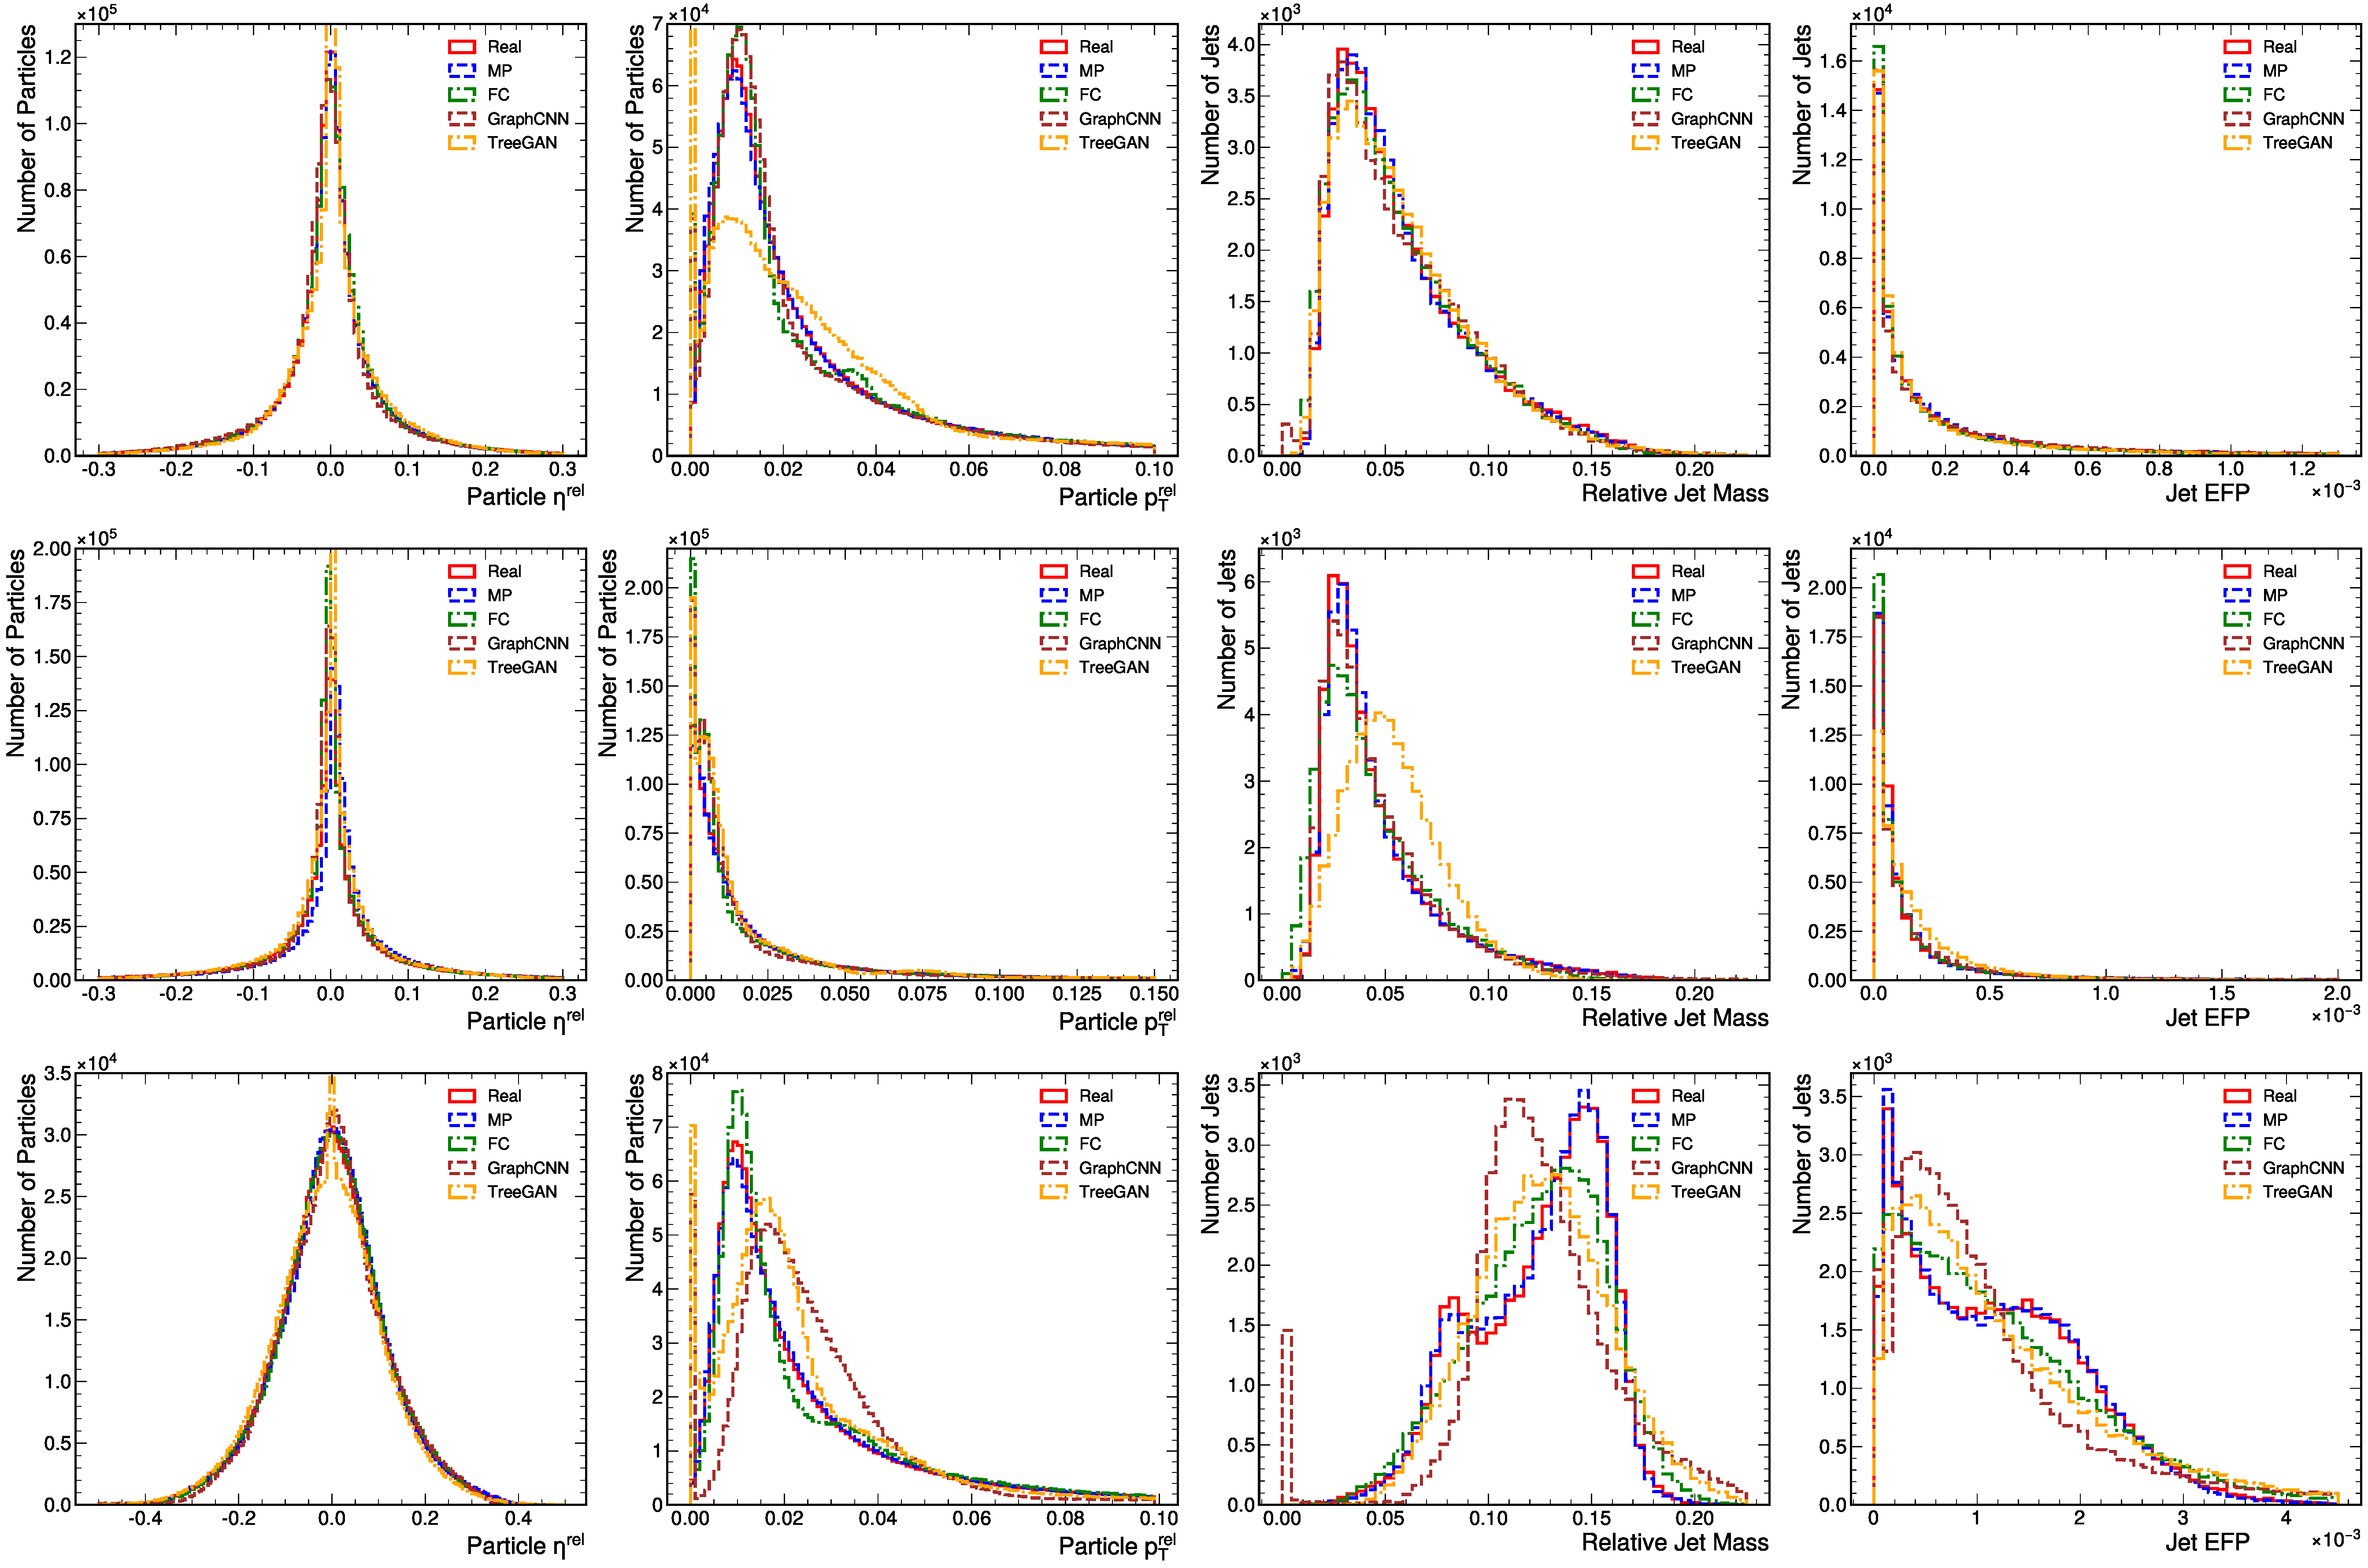
\includegraphics[width=\textwidth]{figures/04-ML4Sim/mpgan/results/feature_distributions.pdf}}
    \caption[Comparison of real and generated distributions for a subset of jet and particle features.]{Comparison of real and generated distributions for a subset of jet and particle features. We use the best performing model for each of the FC, GraphCNN, TreeGAN, and MP generators, as per Table~\ref{tab:04_mpgan_results}. Top: gluon jet features, Middle: light quark jets, Bottom: top quark jets.
    % \TODO{plot rgan and graphcnngan with cut-offs for zero-padded}
    }
    \label{fig:04_mpgan_results}
\end{figure}

We choose model parameters which, during training, yield the lowest \wassm score.
This is because (1) \wass scores between physical features are more relevant for physics applications than the other three metrics, and (2) qualitatively we find it be a better discriminator of model quality than particle features or EFP scores. 
Table \ref{tab:04_mpgan_results} lists the scores for each model and class, and Figure~\ref{fig:04_mpgan_results} shows plots of selected feature distributions of real and generated jets, for the best performing FC, GraphCNN, TreeGAN, and MP generators.
We also provide discretized images in the angular-coordinates-plane, a.k.a ``jet images'', in Figures~\ref{fig:04_mpgan_jetims_g}---\ref{fig:04_mpgan_jetims_t}; however, we note that it is in general not easy to visually evaluate the quality of individual particle clouds, hence we focus on metrics and visualizations aggregated over batches of clouds.
Overall we find that MPGAN is a significant improvement over the best FC, GraphCNN, and TreeGAN models, particularly for top and light quark jets.
This is evident both visually and quantitatively in every metric, especially jet $\wass$s and FPND, with the exception of \wassp where only the FC generator and PointNet discriminator (FC + PointNet) combination is more performant. 

\begin{table}[htpb!]
\caption{Six evaluation scores on different generator and discriminator combinations. 
Lower is better for all metrics except COV. 
\label{tab:04_mpgan_results}}
\centering\resizebox{\textwidth}{!}{
    \begin{tabular}{cllcccccc}
    \toprule
    Jet class & Generator & Discriminator & 
    \begin{tabular}[c]{@{}l@{}}\wassm \\ ($\times 10^{-3}$)\end{tabular} &
    \begin{tabular}[c]{@{}l@{}}\wassp \\ ($\times 10^{-3}$)\end{tabular} &
    \begin{tabular}[c]{@{}l@{}}\wassefp \\ ($\times 10^{-5}$)\end{tabular} & 
    FPND & COV $\uparrow$ & MMD \\
    \midrule
    \multirow{13}{*}{Gluon}  
     & FC & FC & $18.3 \pm 0.2$ & $9.6 \pm 0.4$ & $8.5 \pm 0.5$ & $176$ & $0.24$ & $0.045$\\ 
 & GraphCNN & FC & $2.6 \pm 0.2$ & $9.6 \pm 0.3$ & $12 \pm 8$ & $61$ & $0.39$ & $0.046$\\ 
 & TreeGAN & FC & $41.9 \pm 0.3$ & $69.3 \pm 0.3$ & $14.2 \pm 0.8$ & $355$ & $0.19$ & $0.130$\\ 
 & FC & PointNet & $1.3 \pm 0.4$ & $1.3 \pm 0.2$ & $1.5 \pm 0.9$ & $5.0$ & $0.49$ & $0.039$\\ 
 & GraphCNN & PointNet & $1.9 \pm 0.2$ & $16 \pm 6$ & $200 \pm 1000$ & $7$k & $0.46$ & $0.040$\\ 
 & TreeGAN & PointNet & $1.7 \pm 0.1$ & $4.0 \pm 0.4$ & $4 \pm 1$ & $84$ & $0.37$ & $0.042$\\ 
\cmidrule(lr){2-3}
 & MP & MP & $0.7 \pm 0.2$ & $\mathbf{0.9 \pm 0.3}$ & $\mathbf{0.7 \pm 0.2}$ & $\mathbf{0.12}$ & $\mathbf{0.56}$ & $0.037$\\ 
 & MP-LFC & MP & $\mathbf{0.69 \pm 0.07}$ & $1.8 \pm 0.2$ & $0.9 \pm 0.6$ & $0.20$ & $0.54$ & $0.037$\\ 
\cmidrule(lr){2-3}
 & FC & MP & $4.3 \pm 0.3$ & $21.1 \pm 0.2$ & $9 \pm 1$ & $368$ & $0.11$ & $0.085$\\ 
 & GraphCNN & MP & $2.5 \pm 0.1$ & $9.8 \pm 0.2$ & $13 \pm 8$ & $61$ & $0.38$ & $0.048$\\ 
 & TreeGAN & MP & $2.4 \pm 0.2$ & $12 \pm 7$ & $18 \pm 9$ & $69$ & $0.34$ & $0.048$\\ 
 & MP & FC & $1.2 \pm 0.2$ & $3.7 \pm 0.5$ & $1.6 \pm 0.8$ & $39$ & $0.44$ & $0.040$\\ 
 & MP & PointNet & $1.3 \pm 0.4$ & $1.2 \pm 0.4$ & $4 \pm 2$ & $18$ & $0.53$ & $\mathbf{0.036}$ 
    \\ \midrule
    \multirow{13}{*}{\begin{tabular}[c]{@{}l@{}}Light \\ quark\end{tabular}} 
     & FC & FC & $6.0 \pm 0.2$ & $16.3 \pm 0.9$ & $3.9 \pm 0.6$ & $395$ & $0.18$ & $0.053$\\
 & GraphCNN & FC & $3.5 \pm 0.2$ & $15.1 \pm 0.4$ & $10 \pm 50$ & $100$ & $0.25$ & $0.038$\\
 & TreeGAN & FC & $31.5 \pm 0.3$ & $22.3 \pm 0.4$ & $9.3 \pm 0.4$ & $176$ & $0.06$ & $0.055$\\
 & FC & PointNet & $3.1 \pm 0.2$ & $4.5 \pm 0.4$ & $2.3 \pm 0.6$ & $17$ & $0.37$ & $0.028$\\
 & GraphCNN & PointNet & $4 \pm 1$ & $5.2 \pm 0.5$ & $50$k $\pm 100$k & $316$ & $0.37$ & $0.031$\\
 & TreeGAN & PointNet & $10.1 \pm 0.1$ & $5.7 \pm 0.5$ & $4.1 \pm 0.3$ & $11$ & $0.47$ & $0.031$\\
\cmidrule(lr){2-3}
 & MP & MP & $\mathbf{0.6 \pm 0.2}$ & $4.9 \pm 0.5$ & $\mathbf{0.7 \pm 0.4}$ & $0.35$ & $0.50$ & $0.026$\\
 & MP-LFC & MP & $0.7 \pm 0.2$ & $\mathbf{2.6 \pm 0.4}$ & $0.9 \pm 0.9$ & $\mathbf{0.08}$ & $\mathbf{0.52}$ & $\mathbf{0.024}$\\
\cmidrule(lr){2-3}
 & FC & MP & $6.3 \pm 0.2$ & $16.5 \pm 0.2$ & $4.0 \pm 0.8$ & $212$ & $0.11$ & $0.070$\\
 & GraphCNN & MP & $3.5 \pm 0.4$ & $15.0 \pm 0.3$ & $10 \pm 10$ & $99$ & $0.26$ & $0.038$\\
 & TreeGAN & MP & $4.8 \pm 0.2$ & $33 \pm 6$ & $10 \pm 2$ & $148$ & $0.22$ & $0.041$\\
 & MP & FC & $1.3 \pm 0.1$ & $4.5 \pm 0.4$ & $2.2 \pm 0.6$ & $41$ & $0.37$ & $0.030$\\
 & MP & PointNet & $6.5 \pm 0.3$ & $23.2 \pm 0.6$ & $6 \pm 1$ & $850$ & $0.18$ & $0.034$

    \\ \midrule
    \multirow{13}{*}{\begin{tabular}[c]{@{}l@{}}Top \\ quark\end{tabular}} 
     & FC & FC & $4.8 \pm 0.3$ & $14.5 \pm 0.6$ & $23 \pm 3$ & $160$ & $0.28$ & $0.103$\\
 & GraphCNN & FC & $7.0 \pm 0.3$ & $8.0 \pm 0.5$ & $1$k $\pm 6$k & $15$ & $0.48$ & $0.081$\\
 & TreeGAN & FC & $17.0 \pm 0.2$ & $19.6 \pm 0.6$ & $33 \pm 2$ & $77$ & $0.39$ & $0.083$\\
 & FC & PointNet & $2.7 \pm 0.1$ & $\mathbf{1.6 \pm 0.4}$ & $7.7 \pm 0.5$ & $3.9$ & $0.56$ & $0.075$\\
 & GraphCNN & PointNet & $11.3 \pm 0.9$ & $30 \pm 10$ & $37 \pm 2$ & $30$k & $0.39$ & $0.085$\\
 & TreeGAN & PointNet & $5.19 \pm 0.08$ & $9.1 \pm 0.3$ & $16 \pm 2$ & $17$ & $0.53$ & $0.079$\\
\cmidrule(lr){2-3}
 & MP & MP & $\mathbf{0.6 \pm 0.2}$ & $2.3 \pm 0.3$ & $\mathbf{2 \pm 1}$ & $\mathbf{0.37}$ & $0.57$ & $\mathbf{0.071}$\\
 & MP-LFC & MP & $0.9 \pm 0.3$ & $2.2 \pm 0.7$ & $\mathbf{2 \pm 1}$ & $0.93$ & $0.56$ & $0.073$\\
\cmidrule(lr){2-3}
 & FC & MP & $6.9 \pm 0.1$ & $39.1 \pm 0.3$ & $15 \pm 1$ & $81$ & $0.26$ & $0.120$\\
 & GraphCNN & MP & $6.7 \pm 0.1$ & $8.2 \pm 0.5$ & $40 \pm 10$ & $15$ & $0.49$ & $0.081$\\
 & TreeGAN & MP & $13.4 \pm 0.4$ & $45 \pm 7$ & $50 \pm 30$ & $66$ & $0.29$ & $0.101$\\
 & MP & FC & $12.9 \pm 0.3$ & $26.3 \pm 0.4$ & $46 \pm 3$ & $58$ & $0.27$ & $0.103$\\
 & MP & PointNet & $0.76 \pm 0.08$ & $\mathbf{1.6 \pm 0.4}$ & $4 \pm 1$ & $3.7$ & $\mathbf{0.59}$ & $0.072$

    \\ \midrule
    \end{tabular}
}
\end{table}


\begin{figure}[htpb]
    \centering
    \centerline{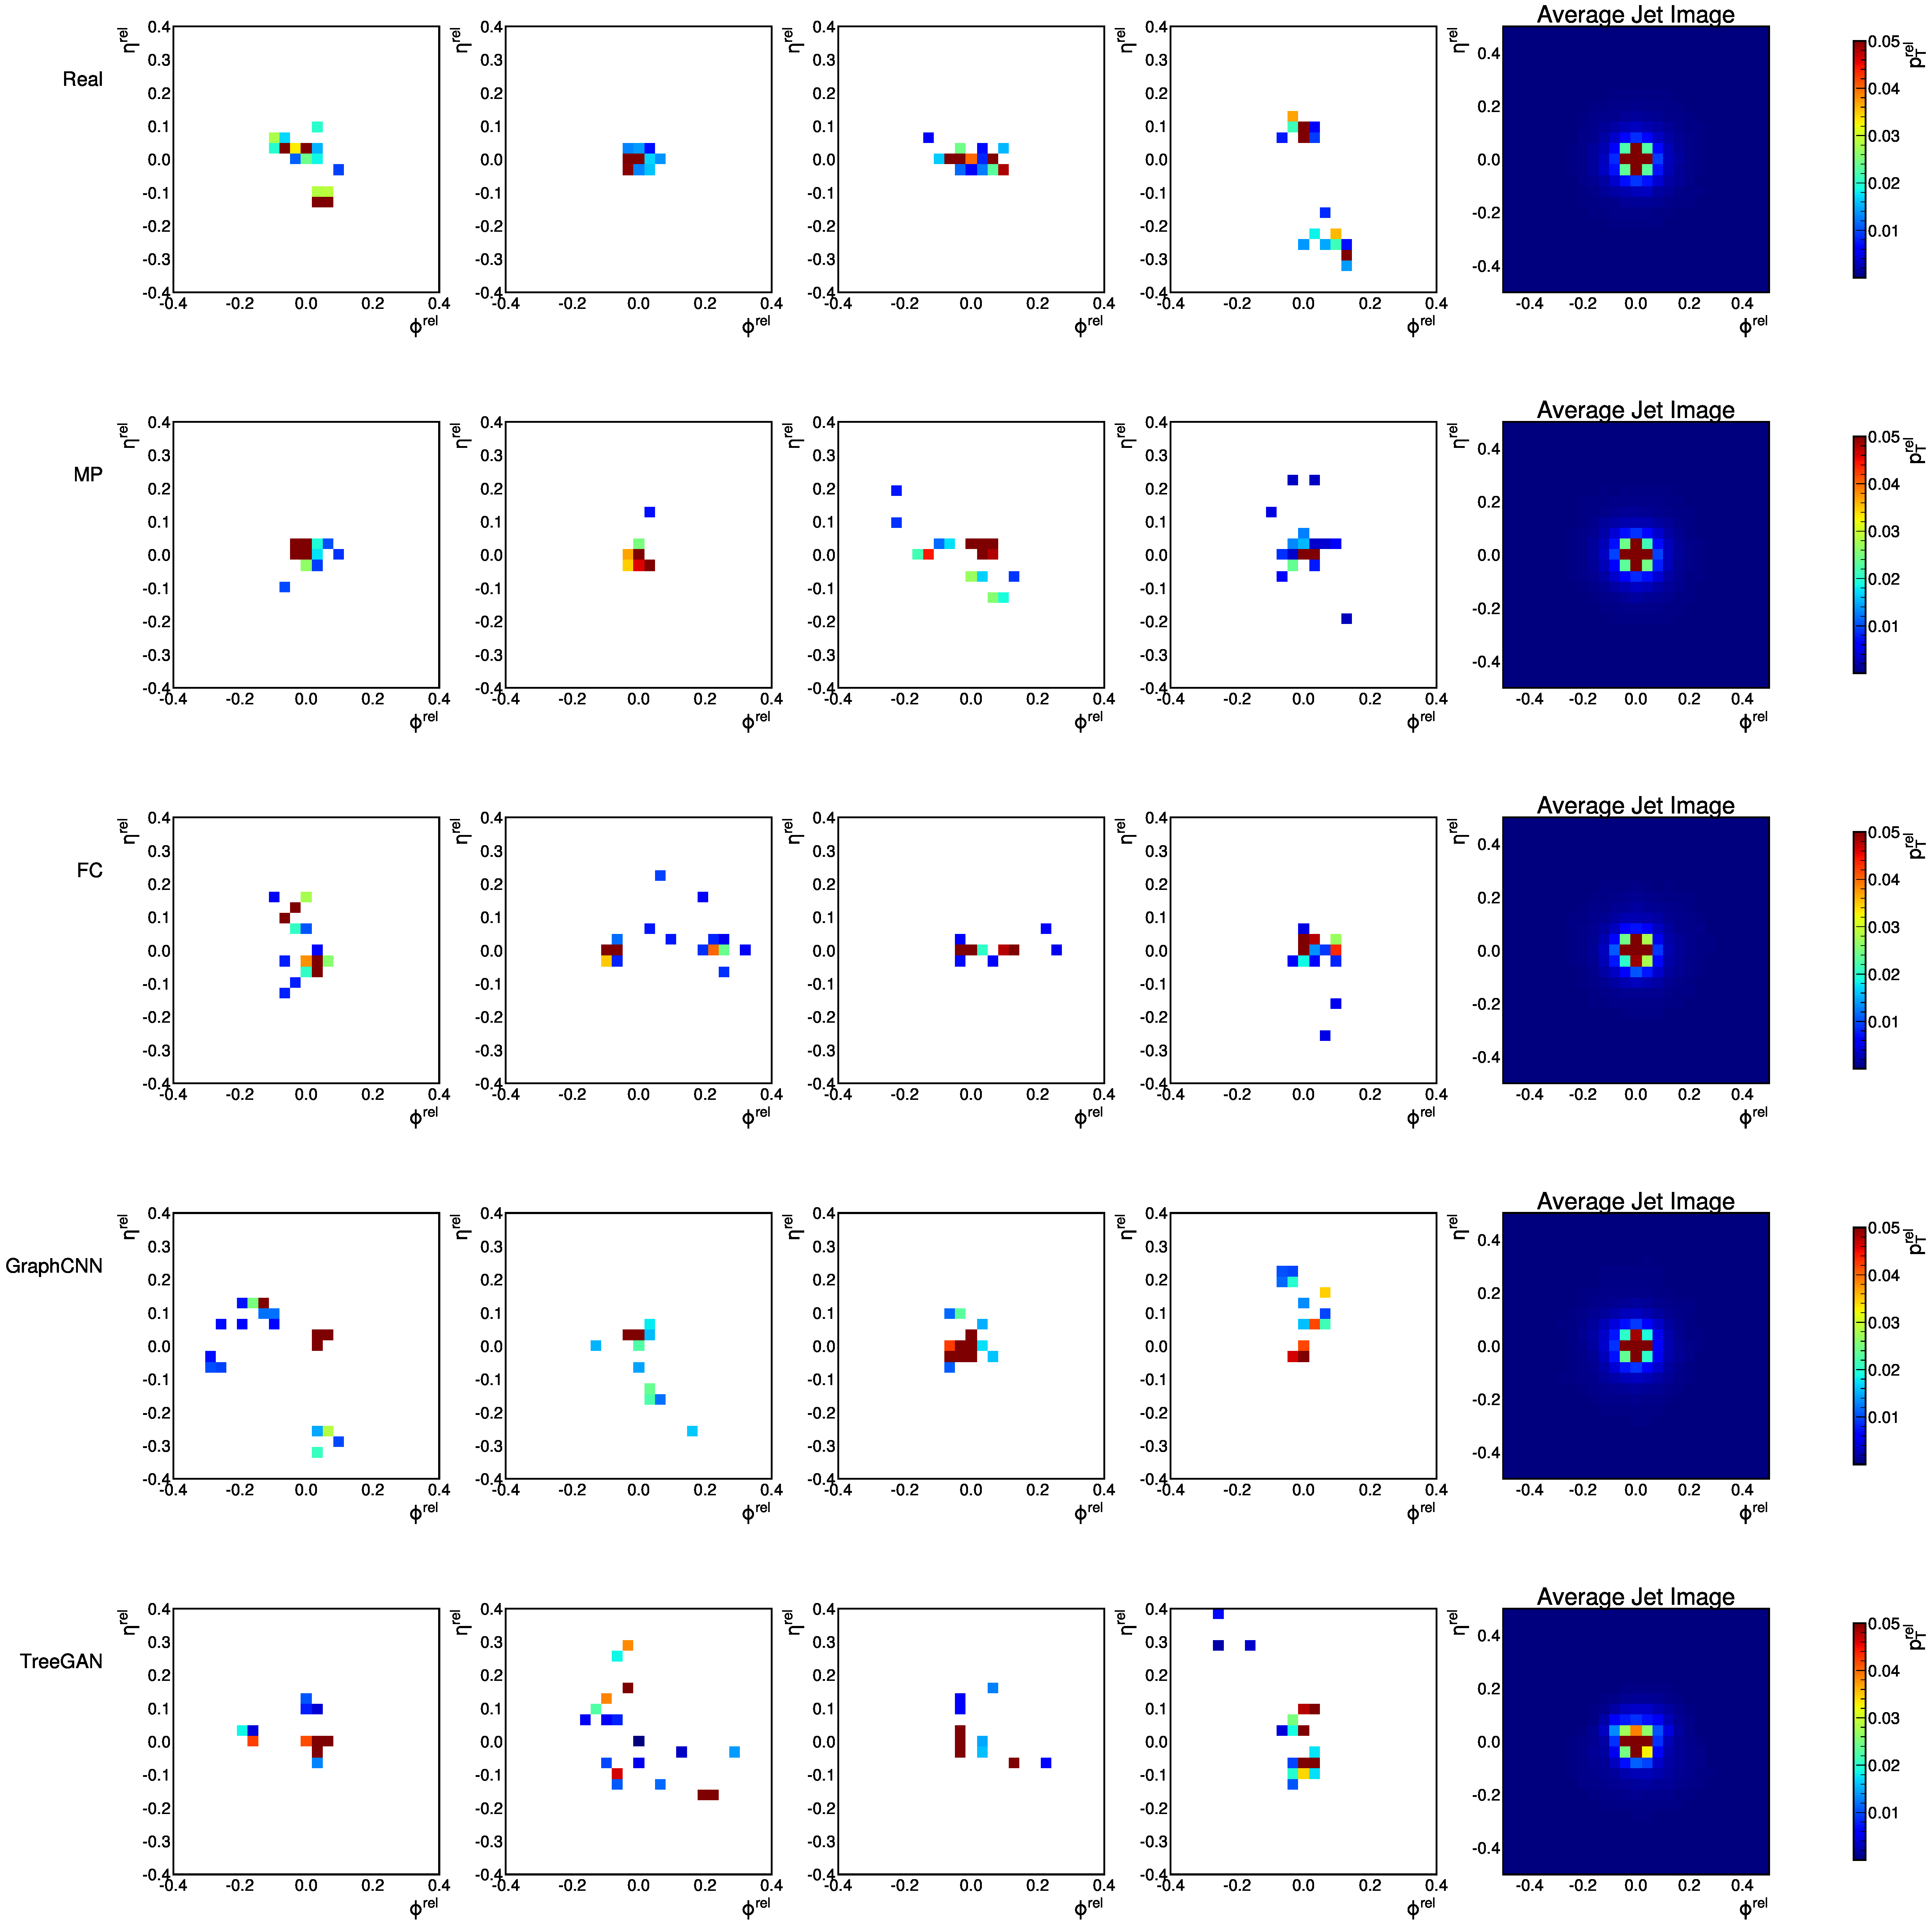
\includegraphics[width=\textwidth]{figures/04-ML4Sim/mpgan/results/jet_images_g.pdf}}
    \caption{Random samples of discretized images in the \etarel$-$\phirel plane, with pixel intensities equal to particle \ptrel, of real and generated gluon jets (left), and an average over 10,000 such sample images (right).}
    \label{fig:04_mpgan_jetims_g}
\end{figure}

\begin{figure}[htpb]
    \centering
    \centerline{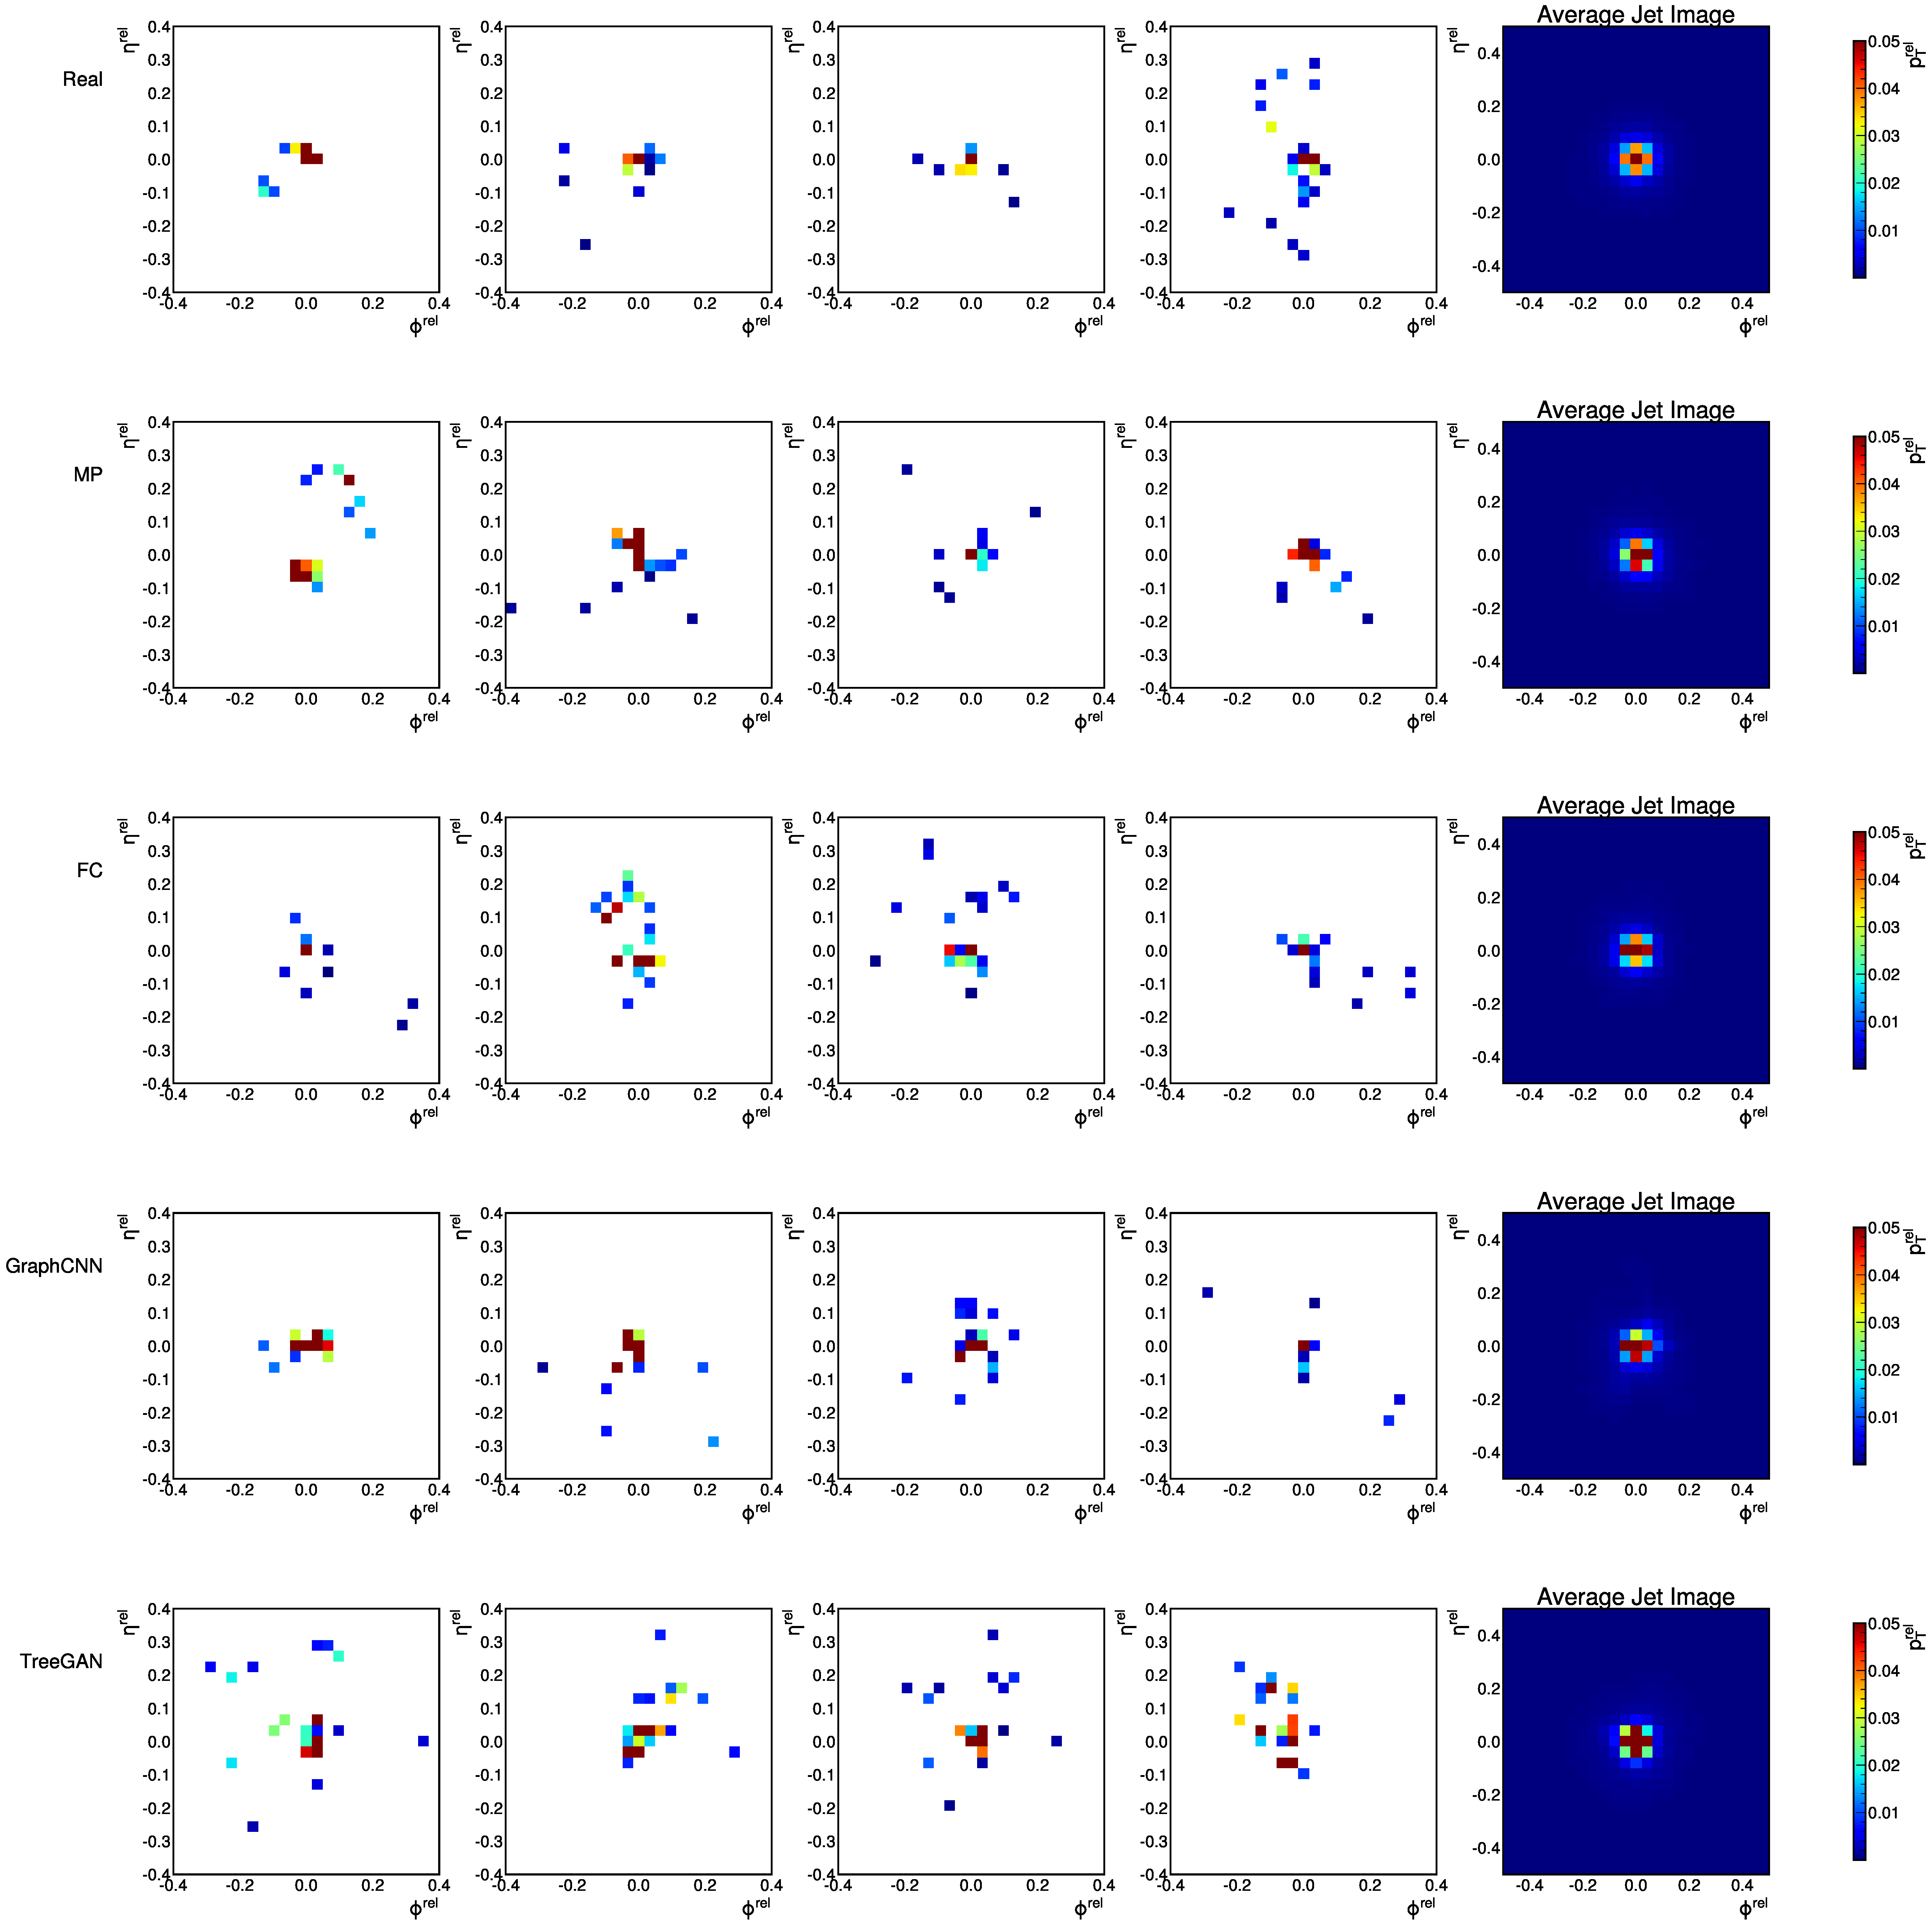
\includegraphics[width=\textwidth]{figures/04-ML4Sim/mpgan/results/jet_images_q.pdf}}
    \caption{Random samples of discretized images in the \etarel$-$\phirel plane, with pixel intensities equal to particle \ptrel, of real and generated light quark jets (left), and an average over 10,000 such sample images (right).}
    \label{fig:04_mpgan_jetims_q}
\end{figure}

\begin{figure}[htpb]
    \centering
    \centerline{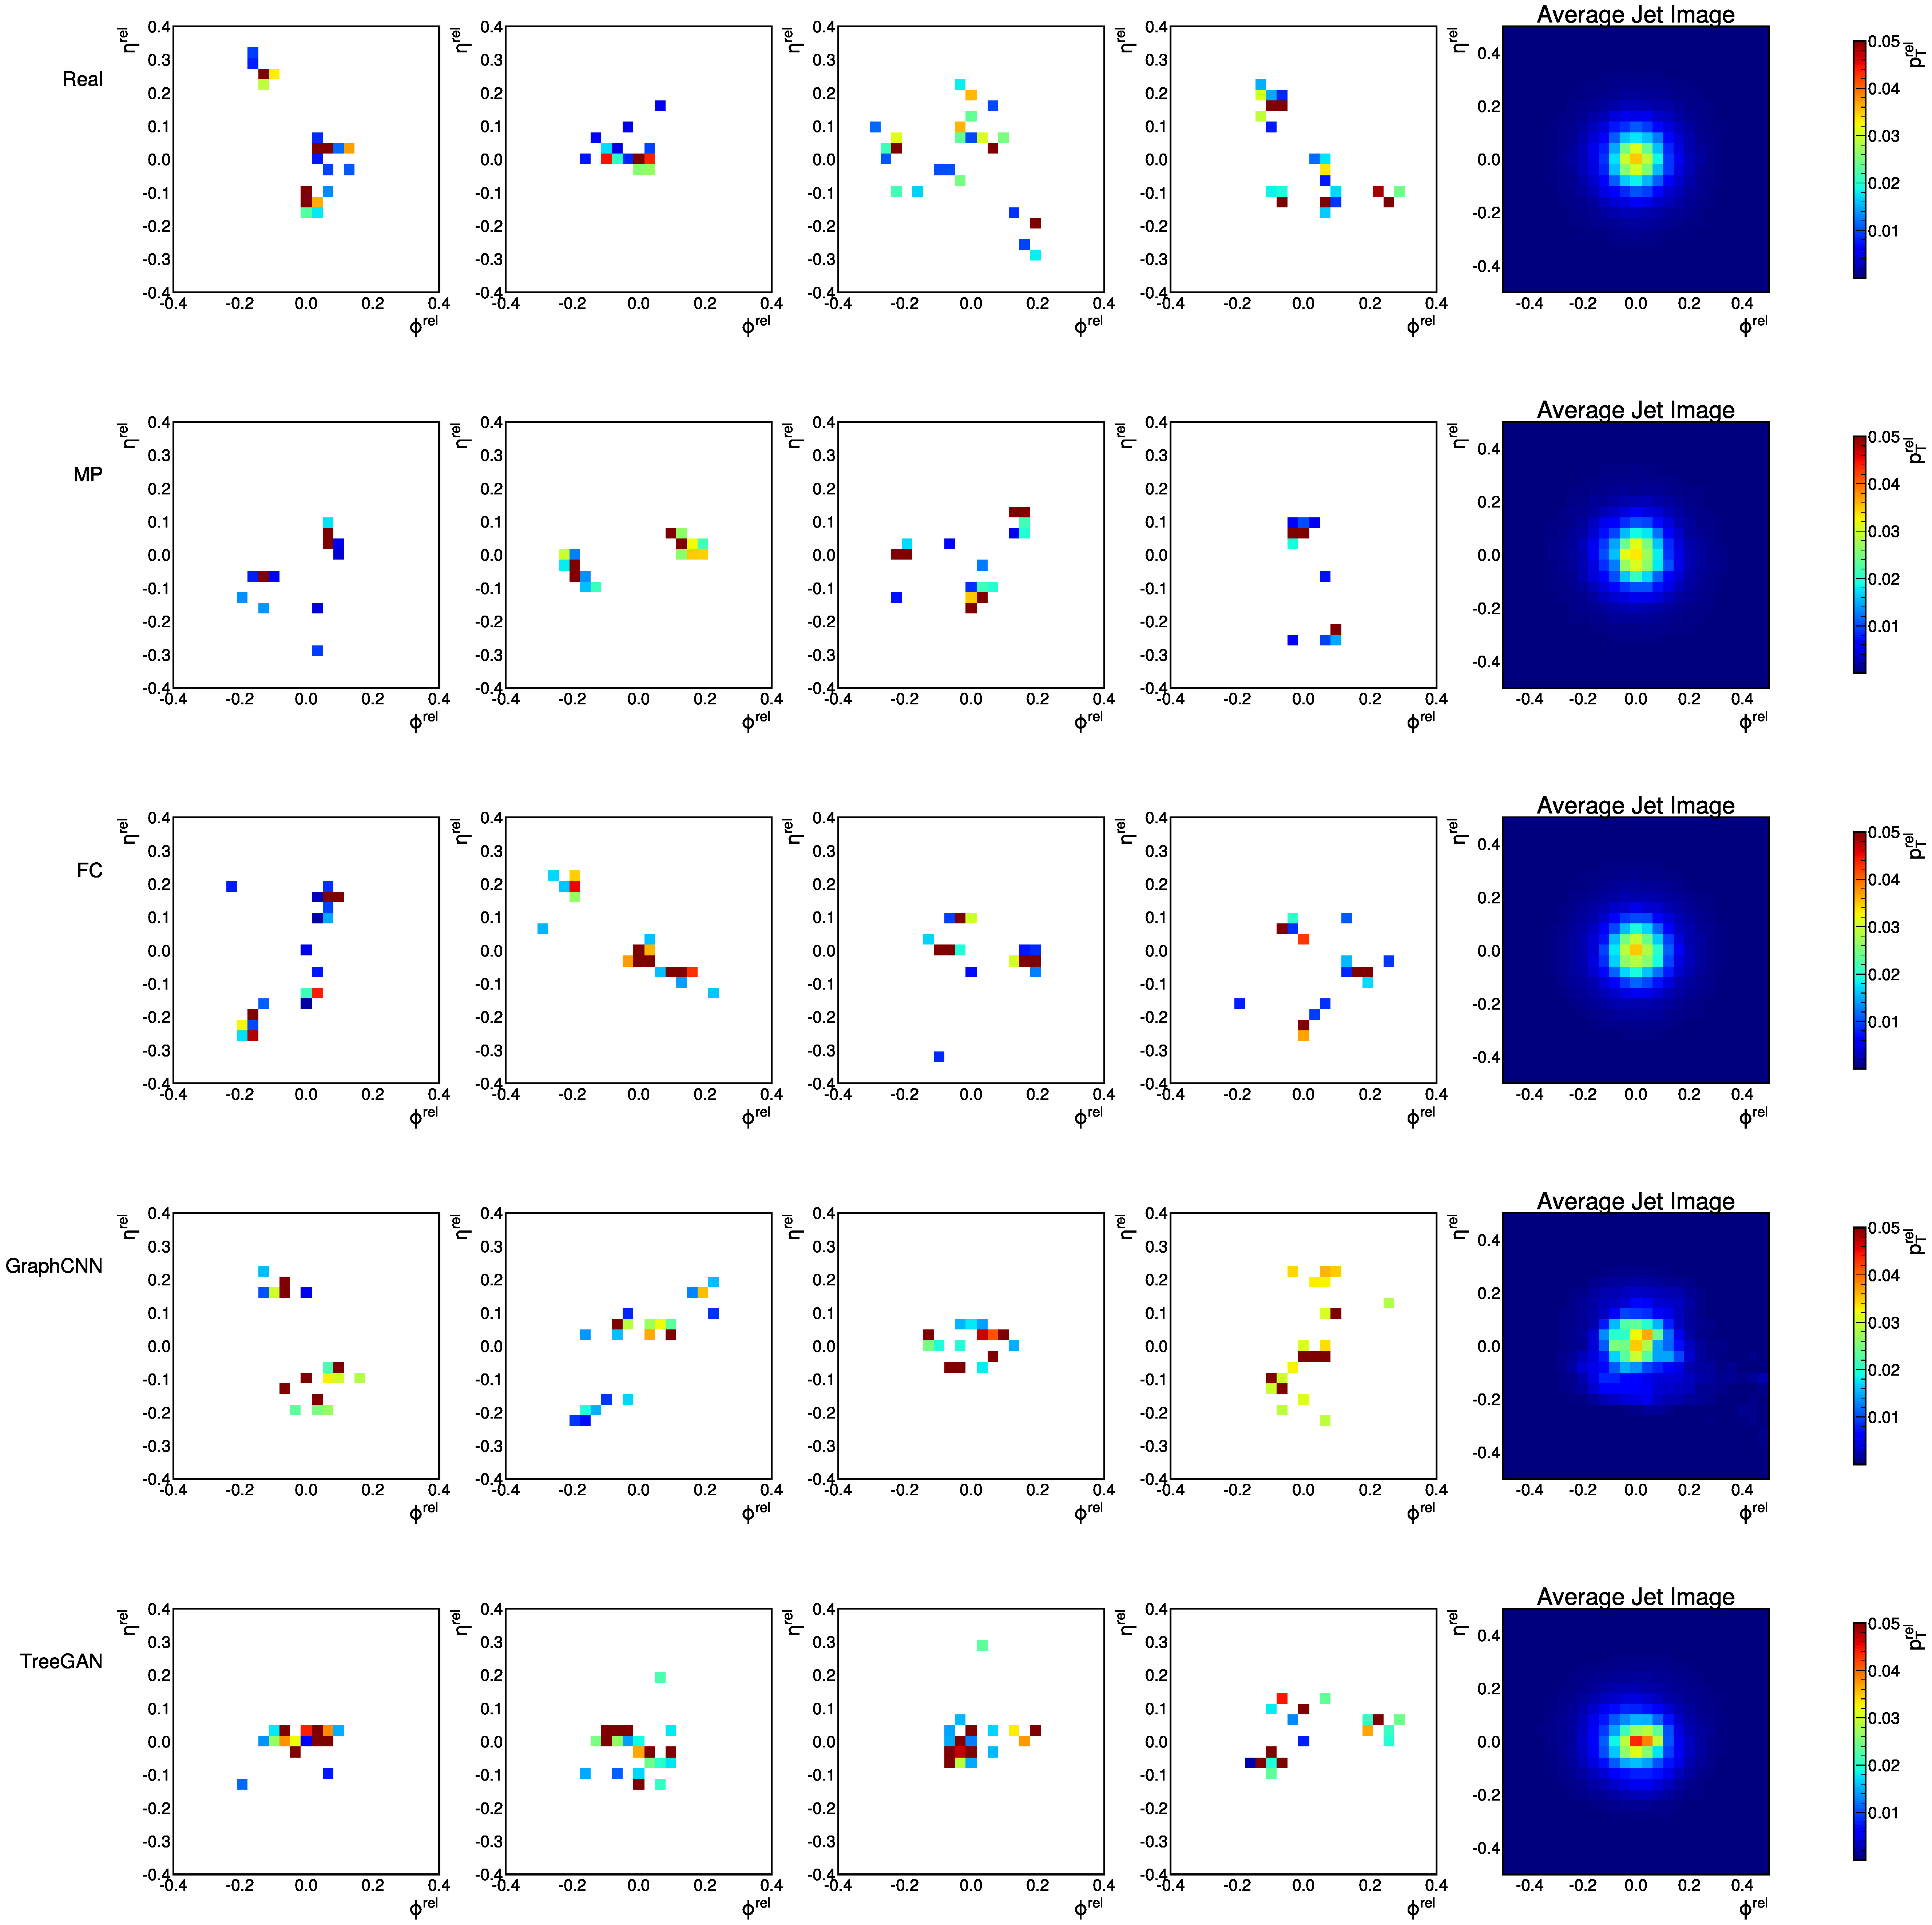
\includegraphics[width=\textwidth]{figures/04-ML4Sim/mpgan/results/jet_images_t.pdf}}
    \caption{Random samples of discretized images in the \etarel$-$\phirel plane, with pixel intensities equal to particle \ptrel, of real and generated top quark jets (left), and an average over 10,000 such sample images (right).}
    \label{fig:04_mpgan_jetims_t}
\end{figure}

We additionally perform a latency measurement and find, using an NVIDIA A100 GPU, that MPGAN generation requires $35.7\mu$s per jet. 
In comparison, the traditional generation process for \jetnet is measured on an 8-CPU machine as requiring 46ms per jet, meaning MPGAN provides a three-orders-of-magnitude speed-up.
Furthermore, as noted in Section~\ref{sec:04_jetnet_dataset}, the generation of \jetnet is significantly simpler than full simulation and reconstruction used at the LHC, which has been measured to require 12.3s~\cite{Pedro:2018jqu} and 4s~\cite{chen2020data} respectively per top quark jet. 
Hence in practical applications we anticipate MPGAN's improvement to potentially rise to five-orders-of-magnitude.


\subsubsection{Real baseline comparison}

We find that MPGAN's jet-level \wass scores all fall within error of the baselines in Table~\ref{tab:04_mpgan_realw1}, while those of alternative generators are several standard deviations away. 
% best performing fc gen is ~4x worse on top jet features
This is particularly an issue with complex top quark particle clouds, where we can see in Figure~\ref{fig:04_mpgan_results} none of the existing generators are able to learn the bimodal jet feature distributions, and smaller light quark clouds, where we see distortion of jet features due to difficulty reproducing the zero-padded particle features. 
No model is able to achieve particle-level scores close to the baseline, and only those of the FC + PointNet combination and MPGAN are of the same order of magnitude.
We conclude that MPGAN reproduces the physical observable distributions to the highest degree of accuracy, but note, however, that it requires further improvement in particle feature reconstruction before it is ready for practical application in HEP.

\subsubsection{Architecture discussion}

To disentangle the effectiveness of the MP generator and discriminator, we train each individually with alternative counterparts (Table~\ref{tab:04_mpgan_results}). 
With the same PointNet discriminator, the GraphCNN and TreeGAN generators perform worse than the simple FC generator for every metric on all three datasets.
The physics-motivated MP generator on the other hand outperforms all on the gluon and top quark datasets, and significantly so on the jet-level \wass scores and the FPND. 
We note, however, that the MP generator is not a significant improvement over the other generators with an FC discriminator. 
Holding the generator fixed, the PointNet discriminator performs significantly better over the FC for all metrics.
With the FC, GraphCNN, and TreeGAN generators, PointNet is also an improvement over the MP discriminator.
With an MP generator, the MP discrimimator is more performant on jet-level \wass and FPND scores but, on the top quark dataset, degrades \wassp relative to PointNet.

We learn from these three things: (1) a generator or discriminator architecture is only as effective as its counterpart---even though the MPGAN combination is the best overall, when paired with a network which is not able to learn complex substructure, or which breaks the permutation symmetry, neither the generator or discriminator is performant, (2) for high-fidelity jet feature reconstruction, both networks must be able to learn complex multi-particle correlations---however, this can come at the cost of low-level feature accuracy, and (3) MPGAN's masking strategy is highly effective as both MP networks are improvements all around on light quark jets.


\subsubsection{Particle cloud evaluation metrics}

\begin{figure}[htpb]
    \centering
    \centerline{
    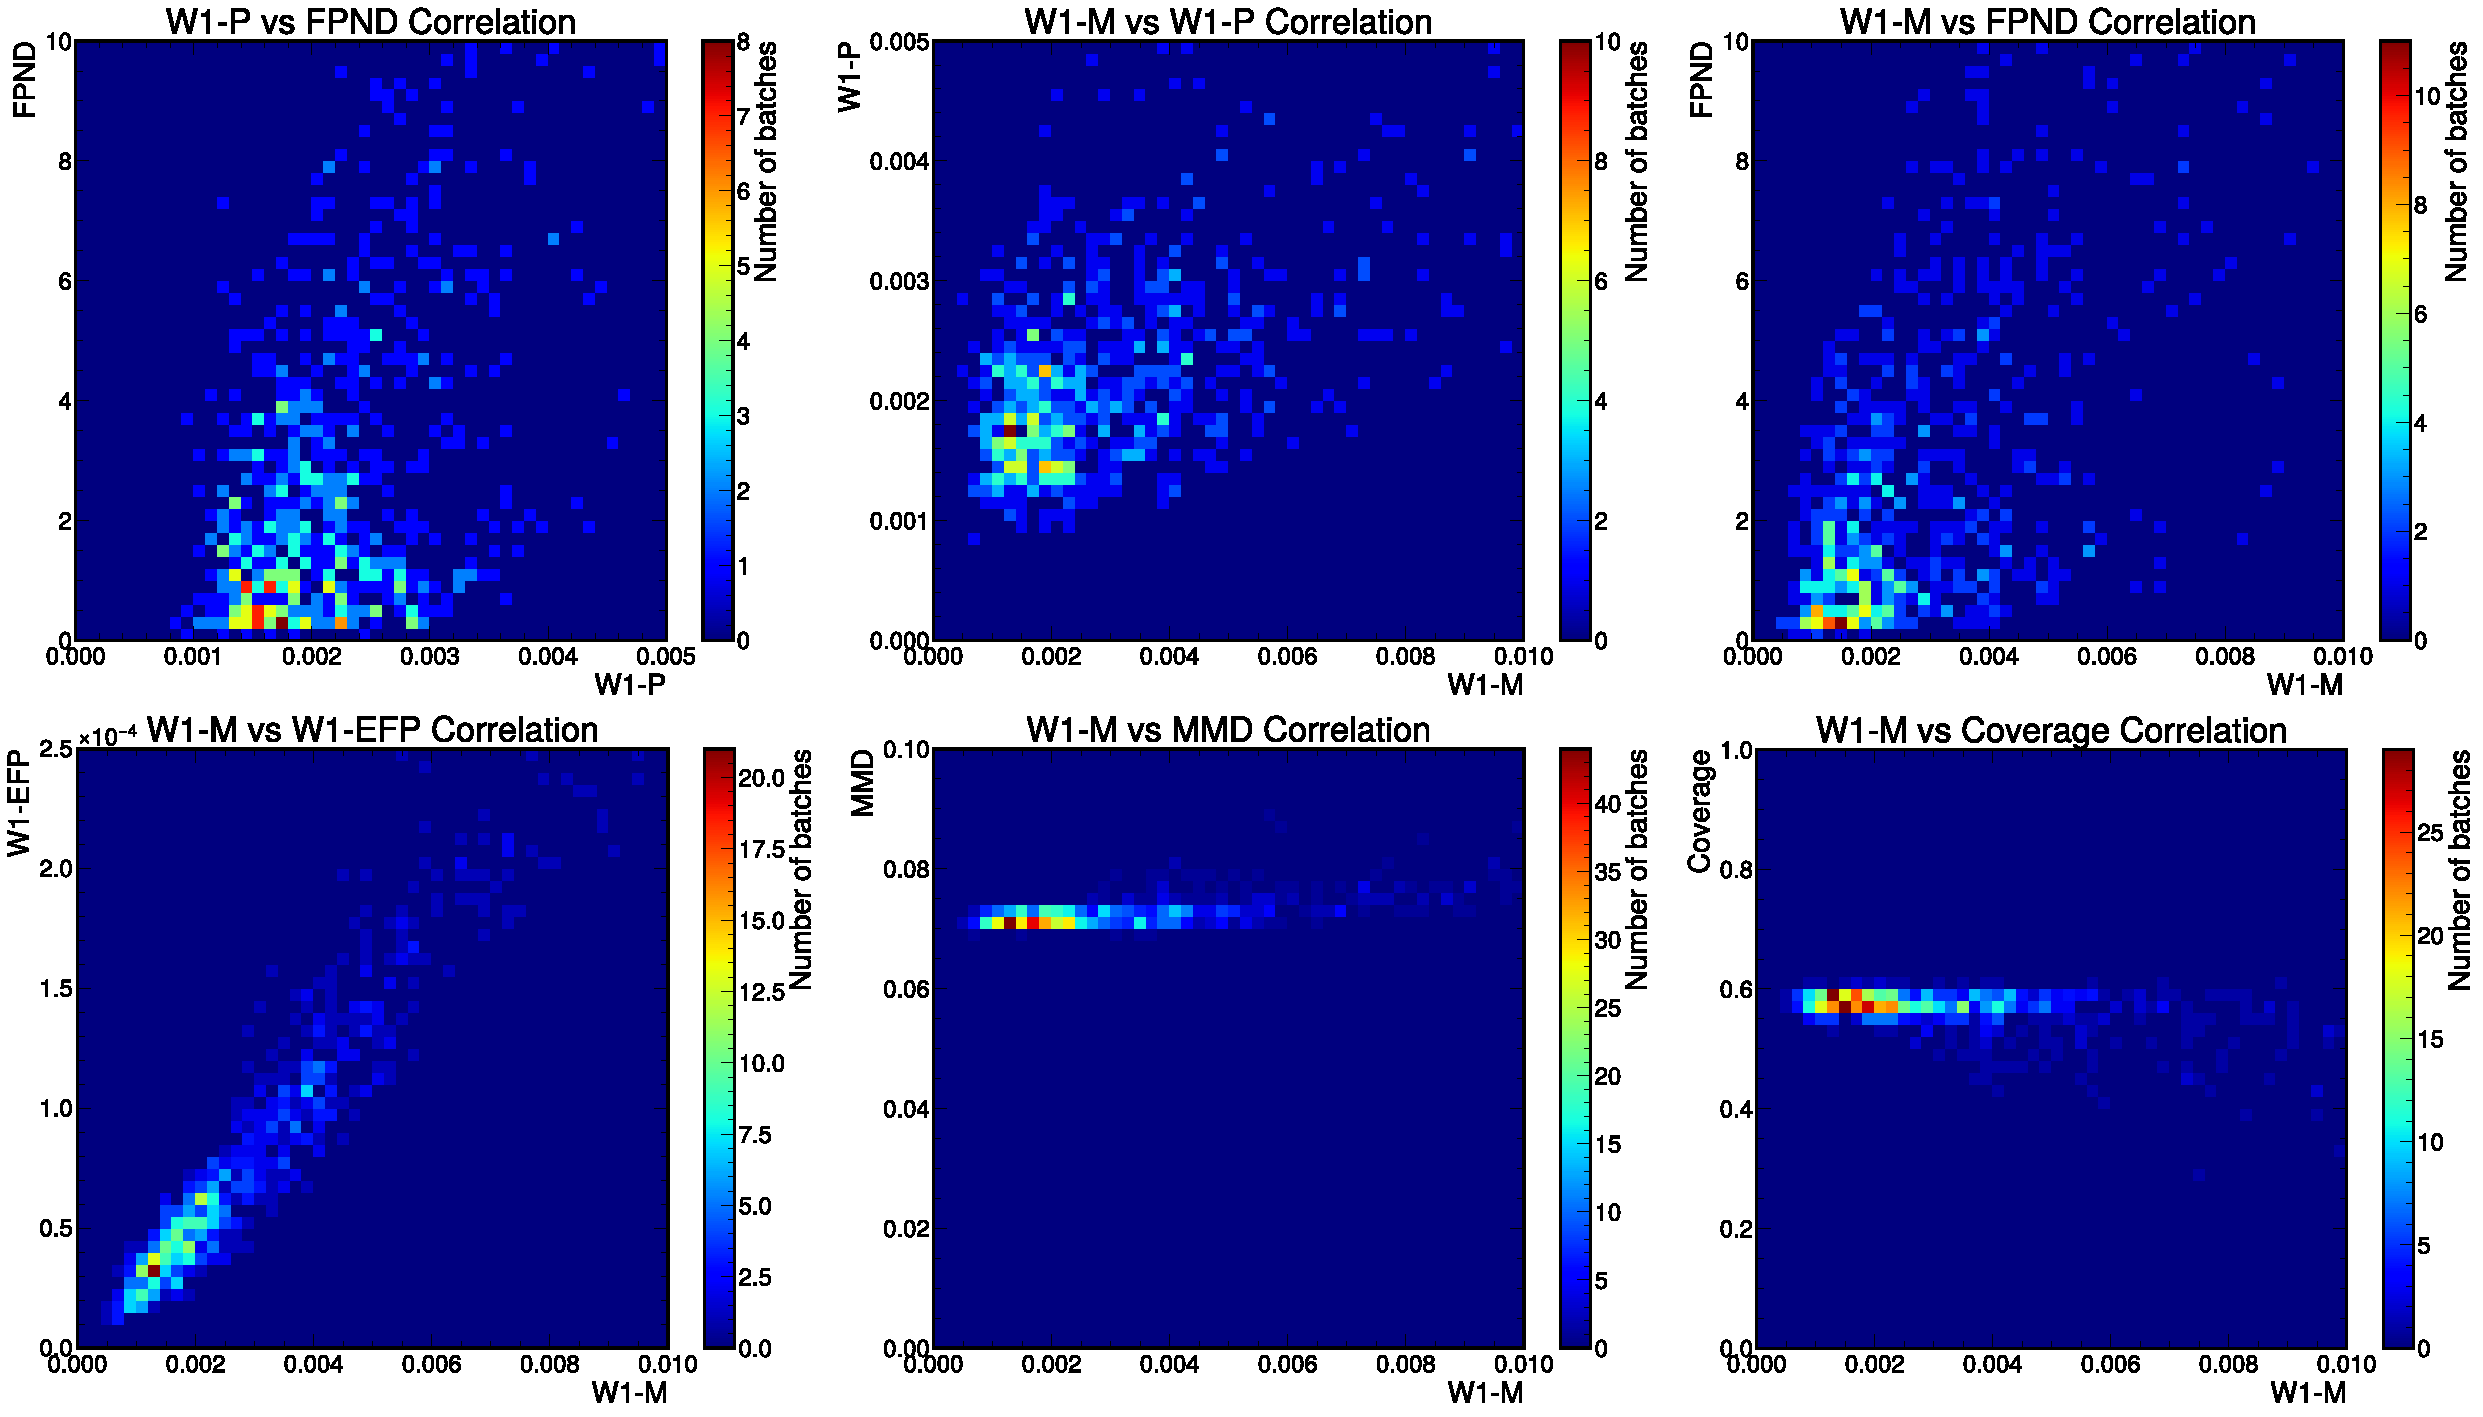
\includegraphics[width=\textwidth]{figures/04-ML4Sim/mpgan/correlation_plots.pdf}}
    \caption{Correlation plots between pairs of evaluation metrics, evaluated on 400 separate batches of 50,000 MPGAN generated top quark jets.
    }
    \label{fig:04_mpgan_correlation}
\end{figure}

We now discuss the merits of each evaluation metrics and provide suggestions for their use in future work. Figure~\ref{fig:04_mpgan_correlation} shows correlation plots between chosen pairs of our evaluation metrics.
As expected, we find W1-M and W1-EFP to be highly correlated,  as they both measure learning of global jet features. 
For rigorous validation we suggest measuring both but for time-sensitive use-cases, such as quick evaluations during model training, W1-M should be sufficient. 
W1-M, FPND, and W1-P are all measuring different aspects of the generation and are relatively uncorrelated. 
We expect FPND overall to be the best and most discriminatory metric for evaluation, as it compares features found by a SOTA classifier to be statistically optimum for characterizing jets, while the W1 scores are valuable for their interpretability. 
Out of these, W1-M/W1-EFP are the most important from a physics-standpoint, as we generally characterize collisions by the high-level features of the output jets, rather than the individual particle features. 

MMD and coverage are both valuable for specifically evaluating the quality and diversity of samples respectively, however we see from Figure~\ref{fig:04_mpgan_correlation} that they saturate after a certain point, after which FPND and \wass scores are necessary for stronger discrimination. 
We also note that in Table~\ref{tab:04_mpgan_results}, models with low \wass scores relative to the baseline have the best coverage and MMD scores as well.
This indicates that the \wass metrics are sensitive to both mode collapse (measured by coverage), which is expected as in terms of feature distributions mode collapse manifests as differing supports, to which the \wass distance is sensitive, as well as to individual sample quality (measured by MMD), which supports our claim that recovering jet feature distributions implies accurate learning of individual cloud structure.
Together this suggests that low \wass scores are able to validate sample quality and against mode collapse, and justifies our criteria that a practical ML simulation alternative have \wass scores close to the baselines in Table~\ref{tab:04_mpgan_results}. 
In conclusion, for thorough validation of generated particle clouds, we recommend considering all three W-1 scores in conjunction with FPND, while MMD and coverage, being focused tests of these aspects of generation, may be useful for understanding failure modes during model development. 


\subsection{Summary}
\label{sec:04_mpgan_summary}

In this section, we applied existing state-of-the-art point cloud generative models to \jetnet, and proposed several physics- and computer-vision-inspired metrics to rigorously evaluate generated clouds.  
We found that existing models are not performant on a number of metrics, and failed to reproduce high-level jet features---arguably the most significant aspect for HEP.
We then introduced the novel message-passing generative adversarial network (MPGAN) model, designed to capture complex global structure and handle variable-sized clouds, which significantly improved performance in this area, as well as other metrics. 

Despite the high performance, the major limitation of MPGAN is the quadratic scaling of the message passing operation, which makes it difficult to scale to larger clouds than 30-particle ones used in Section~\ref{sec:04_mpgan_exp}.
In the next section, we discuss the iGAPT model to overcome this limitation.


\section{Generative adversarial particle transformers}
\label{sec:04_gapt}

In the previous section, we introduced the MPGAN model, which represented a significant advance in ML-based fast simulations for HEP, being able to capture the complex global structure of jets and handle variable-sized particle clouds using fully-connected graph neural networks.
However, this fully-connected nature means its memory and time complexity scale quadratically with the number of particles per jet, leading to difficulty in simulating larger particle clouds.

In this section, we first introduce in Section~\ref{sec:04_gapt_gapt} the generative adversarial particle transformer (GAPT) model, which takes advantage of the computationally efficient ``attention''-mechanism that has led to significant advances in natural language processing.
This provides a significant speed-up over MPGAN, but is still limited by the quadratic scaling of the attention mechanism.
We then present the induced GAPT (iGAPT) model in Section~\ref{sec:04_gapt_igapt}, featuring ``induced particle attention blocks'' (IPABs) that incorporate physics-informed inductive biases of jets, to offer both linear-time complexity and improved output fidelity.
We discuss architecture choices and timing comparisons, but defer a deeper evaluation of the performance of these models and MPGAN to Chapter~\ref{sec:04_evaluating}, which details our new methodology for quantitatively validating and comparing fast simulations.

\subsection{GAPT}
\label{sec:04_gapt_gapt}

Similar to MPGAN, GAPT is a GAN for particle cloud data, but employing self-attention instead of message passing in the two generator and discriminator networks.
It is based on the generative adversarial set transformer (GAST) architecture~\cite{stelzner2020generative}, which makes use of set transformer~\cite{lee2019set} blocks to aggregate information across all points and update their features. 
It maintains the key inductive biases which makes MPGAN successful---permutation symmetry-respecting operations, and fully connected interaction between nodes during generation to learn high-level global features, but with a significant improvement in speed due to the higher computational efficiency of the attention mechanism compared to the message passing operations used in MPGAN.

The generator and discriminator networks are composed of permutation-invariant multihead self-attention blocks (SABs) as defined in Ref.~\cite{lee2019set} and illustrated in Figure~\ref{fig:04_gapt_attention}.
We use four and two SAB blocks in the generator and discriminator respectively.
Each SAB block uses 8 attention heads, and a 128-dimensional embedding space for each of the query, key, and value vectors.
It also contains a one-layer feed-forward neural network (FFN) after each attention step, which maintains the 128-dimensional embedding for node features, and applies a leaky ReLU activation, with negative slope coefficient 0.2.
Residual connections to the pre-SAB node features are used after both the attention step and FFN.
After the final SAB block, a tanh activation is applied to the generator, whereas in the discriminator, the results are first pooled using a pooling by multihead attention (PMA) block~\cite{lee2019set}, followed by a final fully connected layer and sigmoid activation.

For training, we use the mean squared error loss function, as in the LSGAN~\cite{mao_lsgan}, and the RMSProp optimizer with a two timescale update rule~\cite{TTUR}, using a learning rate of $3\cdot10^{-4}$ and $10^{-4}$ for the discriminator and generator respectively.
Dropout, with probability 0.5, is used to regularize the discriminator.
We train for 2000 epochs and select the model with the lowest Fr\'echet physics distance.

\subsection{iGAPT}
\label{sec:04_gapt_igapt}

\begin{figure}[ht]
    \centering
    \captionsetup{justification=centering}
    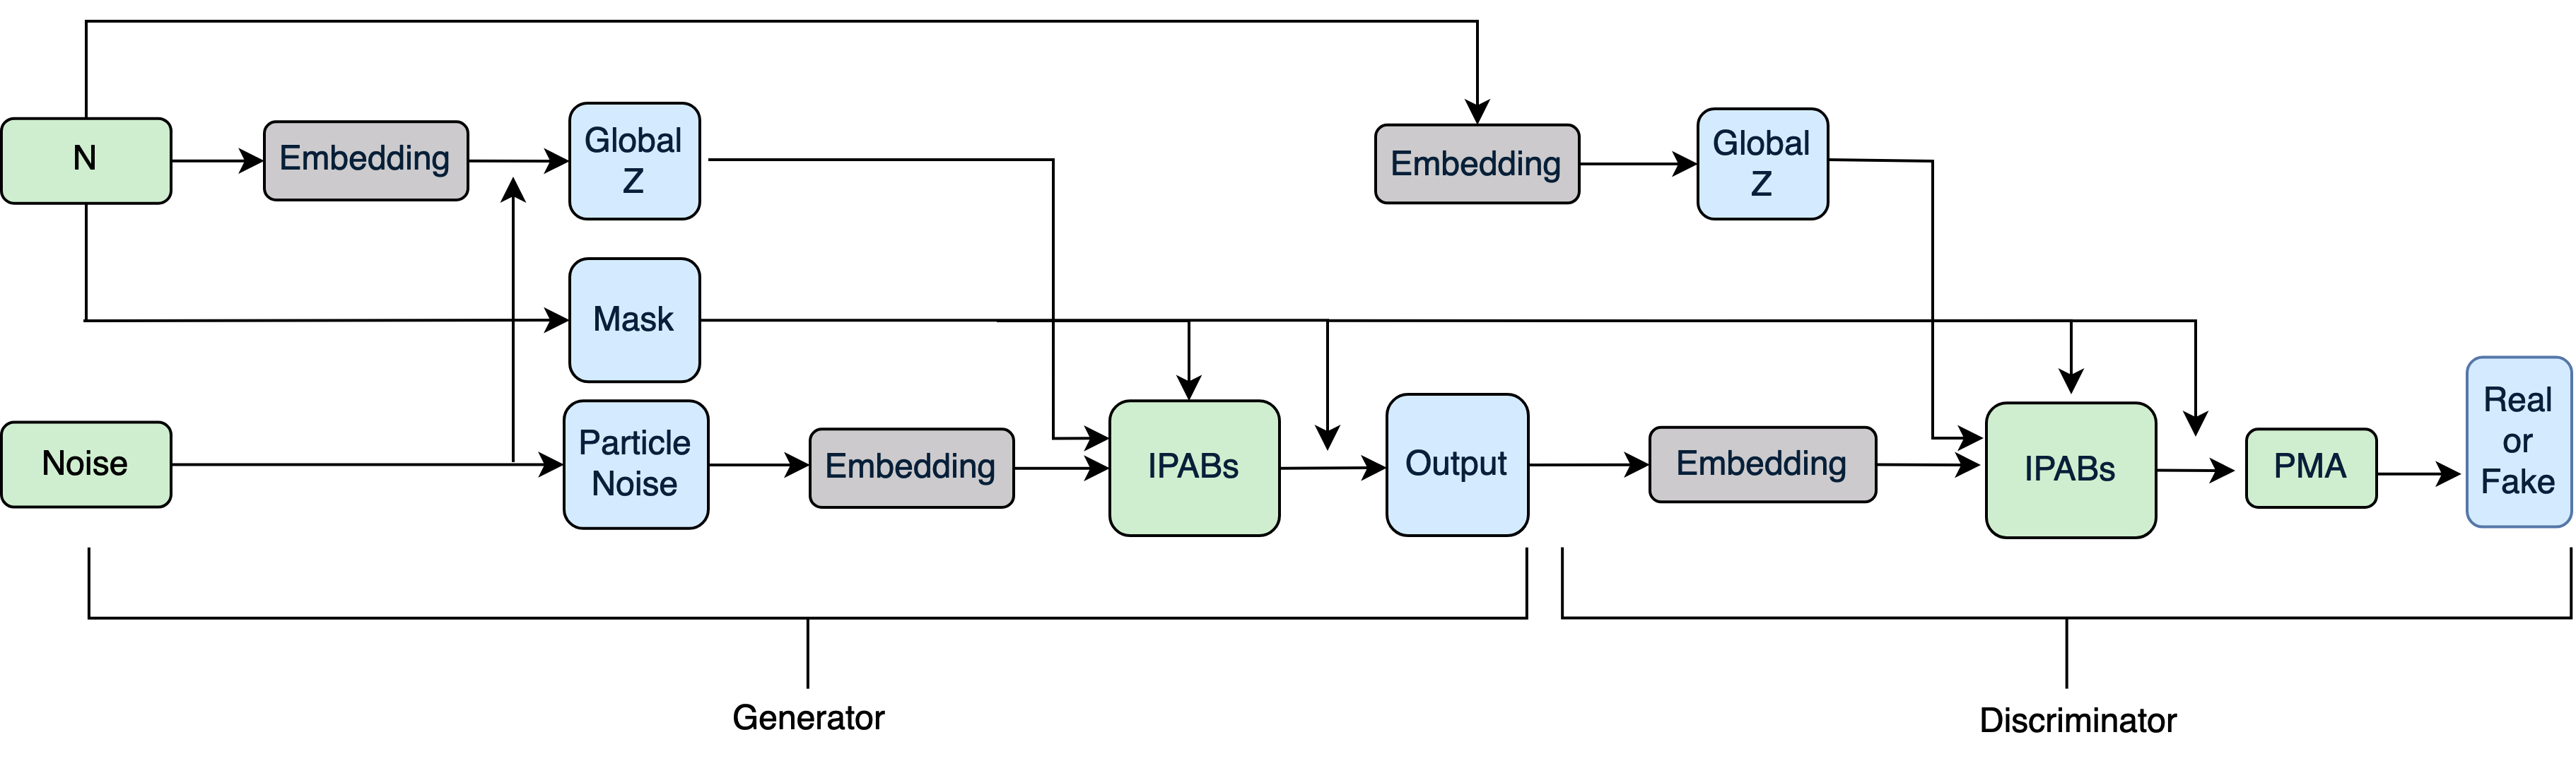
\includegraphics[width=1\linewidth]{figures/04-ML4Sim/igapt/gapt.png}
    \caption{Diagram of the iGAPT generator and discriminator networks.}
    \label{fig:04_igapt_arch}
\end{figure}


The iGAPT model builds on the GAPT architecture, but introduces a novel physics-informed attention mechanism that allows for linear-time complexity in the number of particles per jet.
As illustrated in Figure~\ref{fig:04_igapt_arch}, it is a GAN with the generator and discriminator networks composed of ``induced particle attention blocks'' (IPABs).
On top of maintaining permutation invariance and operating on point-cloud representations, as in MPGAN and GAPT, the key inductive bias we experiment with in iGAPT is maintaining a global vector through the generation and discrimination processes, $\cvec{z}$, which implicitly represents global jet features.
IPABs and different ways of incorporating $\cvec{z}$ into the attention process are described below.

The generation process starts with sampling random Gaussian noise and a particle multiplicity $N$ from the true distribution, which is transformed via a learned linear embedding layer.
The noise has two components: a set of $N_{\mathrm{max}}$ vectors representing initial particle features, and a single vector representing initial jet features.
$N_{\mathrm{max}}$ is the maximum number of particles per jet we want to simulate, and the number of initial particle and jet features is a hyperparameter we tune.
The jet noise is added to the embedded $N$ to produce $\cvec{z}$, which is then transformed along with the particle noise via multiple IPABs to output a generated jet.

The discrimination process starts with a generated or real jet, and the sampled or true jet multiplicity $N$.
This is again transformed via a learned embedding layer to produce the 
$\cvec{z}$ conditioning vector for the discriminator, which along with the input jet are processed through IPABs producing an intermediate jet representation.
The constituents of this jet are aggregated in a permutation-invariant manner using a pooling by multihead attention (PMA) layer, as introduced in~\cite{lee2019set}, the output of which is finally fed into a linear layer to classify the jet as real or fake.

Attention blocks require fixed multiplicity; however, jets naturally have a variable number of particle constituents.
To handle this, we zero-pad all jets to $N_{\mathrm{max}}$ particles and use masked attention in every block to ignore these.


\subsubsection{Attention Blocks}
\label{sec:04_igapt_attentionblocks}

The SAB blocks used by GAPT offer the benefit of global, fully connected interactions between particles; however, this also results in quadratic scaling with the particle multiplicity, which is undesirable.
To counter this, Ref.~\cite{lee2019set} also proposed ``induced'' SABs (ISABs), where the input set is first attended to by $M$ learned inducing vectors via a MAB, outputting an intermediate, compressed representation.
This representation is then attended to by the original set to produce the new output.
This retains the global interactions between particles while achieving $\mathcal O(NM)$ scaling---linear in the particle multiplicity.
ISABs have been used in generative adversarial set transformers (GAST)~\cite{stelzner2020generative}, yielding high quality results on computer vision datasets.
GAST incorporates similar global set features $\cvec{z}$ by concatenating them to each particle before every ISAB operation.

\begin{figure}[ht!]
    \centering
    \captionsetup{justification=centering}
    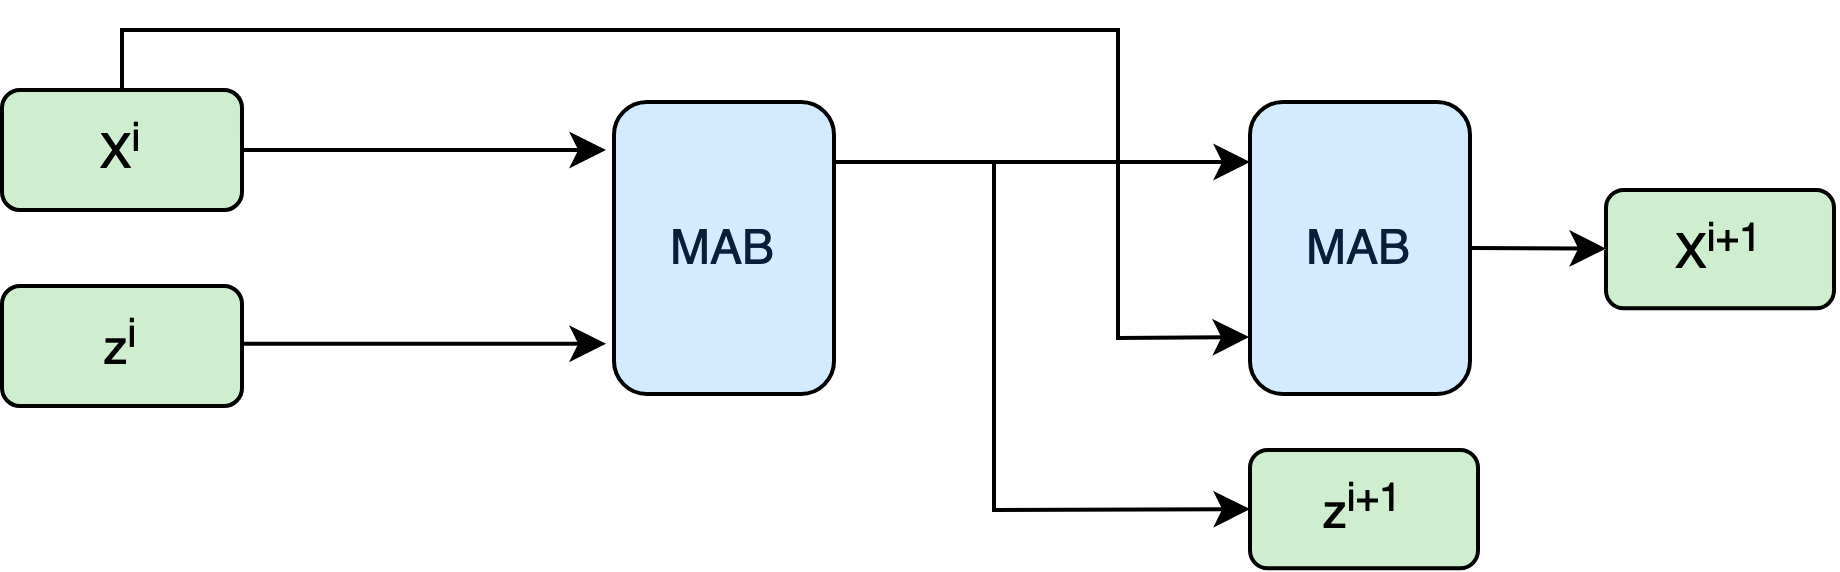
\includegraphics[width=0.7\linewidth]{figures/04-ML4Sim/igapt/IPAB.png}
    \caption{Illustration of an induced particle attention block (IPAB).}
    \label{fig:04_igapt_ipab}
\end{figure}

In iGAPT, we experiment with an alternative version of conditioning, which we call ``induced particle attention''.
Here, $\cvec{z}$ is directly used as the inducing vector in an ISAB, and is continuously updated through the intermediate, induced attention outputs.
Explicitly, as illustrated in Figure~\ref{fig:04_igapt_ipab}, the $i$th IPAB receives as input the jet $\cvec{x}^{i}$ and global features $\cvec{z}^{i}$ from the previous block, after which $\cvec{x}^{i}$ is first attended to by $\cvec{z}^{i}$ to output updated features $\cvec{z}^{i+1}$, and then conversely $\cvec{z}^{i+1}$ is attended to by $\cvec{x}^{i}$ to output the updated jet $\cvec{x}^{i+1}$.
This is interpreted as a way to update and learn the global jet features, such as mass and \pt, along with the individual particle features, and allow both to interact in each attention layer.
An additional and significant advantage is that this induced attention operation involves only one inducing vector --- $\cvec{z}$, hence $M = 1$ and we achieve $\mathcal O(N)$ computational complexity.



\subsubsection{Training and Hyperparameters}

Along with GAPT, we test both the GAST and iGAPT models on the \jetnet dataset, to compare the performance of ISABs and IPABs.
The iGAPT and GAST models were trained for a maximum of 6000 epochs on a single NVIDIA RTX1080 GPU using the RMSProp optimizer.
The training time and batch size for 30- and 150-particle gluon jets is shown in Table~\ref{tab:04_igapt_times_gluon}.
We use a two-time update rule~\cite{TTUR}, with learning rates of $0.5 \times 10^{-4}$ and $1.5 \times 10^{-4}$ for the generator and discriminator, respectively.
The discriminator is regularized with dropout with a probability of 0.5 and layer normalization.
We use a LeakyReLU activation after every linear layer, except the final generator (tanh) and discriminator (sigmoid) outputs.
After hyperparameter tuning, we settle on on 3 and 6 ISAB layers for the generator and discriminator respectively, and 4 and 8 IPAB layers for the iGAPT model.
We use 16 and 128 initial particle and jet features, respectively, in iGAPT.
GAST uses 20 inducing vectors for its ISABs.


\subsection{Experiments}

\subsubsection{Results}

We test and compare the GAPT, GAST, iGAPT, and MPGAN models on 30-particle gluon, light quark, and top quark jets, and on 150-particle gluon jets.
Out of all our trainings, we select the GAPT, GAST, and iGAPT models with the lowest Fr\'{e}chet physics distance score, as will be introduced in Section~\ref{sec:04_evaluating}, due to its high sensitivity to common types of mismodeling.
Comparisons of real and iGAPT- and MPGAN-generated feature distributions are shown in Figure~\ref{fig:04_igapt_feature_distributions_30} and Appendix~\ref{app:04_gapt_150} for 30 and 150 particles, respectively, demonstrating high fidelity results from both models.
We defer a detailed evaluation of the performance to Section~\ref{sec:04_evaluating}.

\begin{figure}[htbp!]
    \centering
    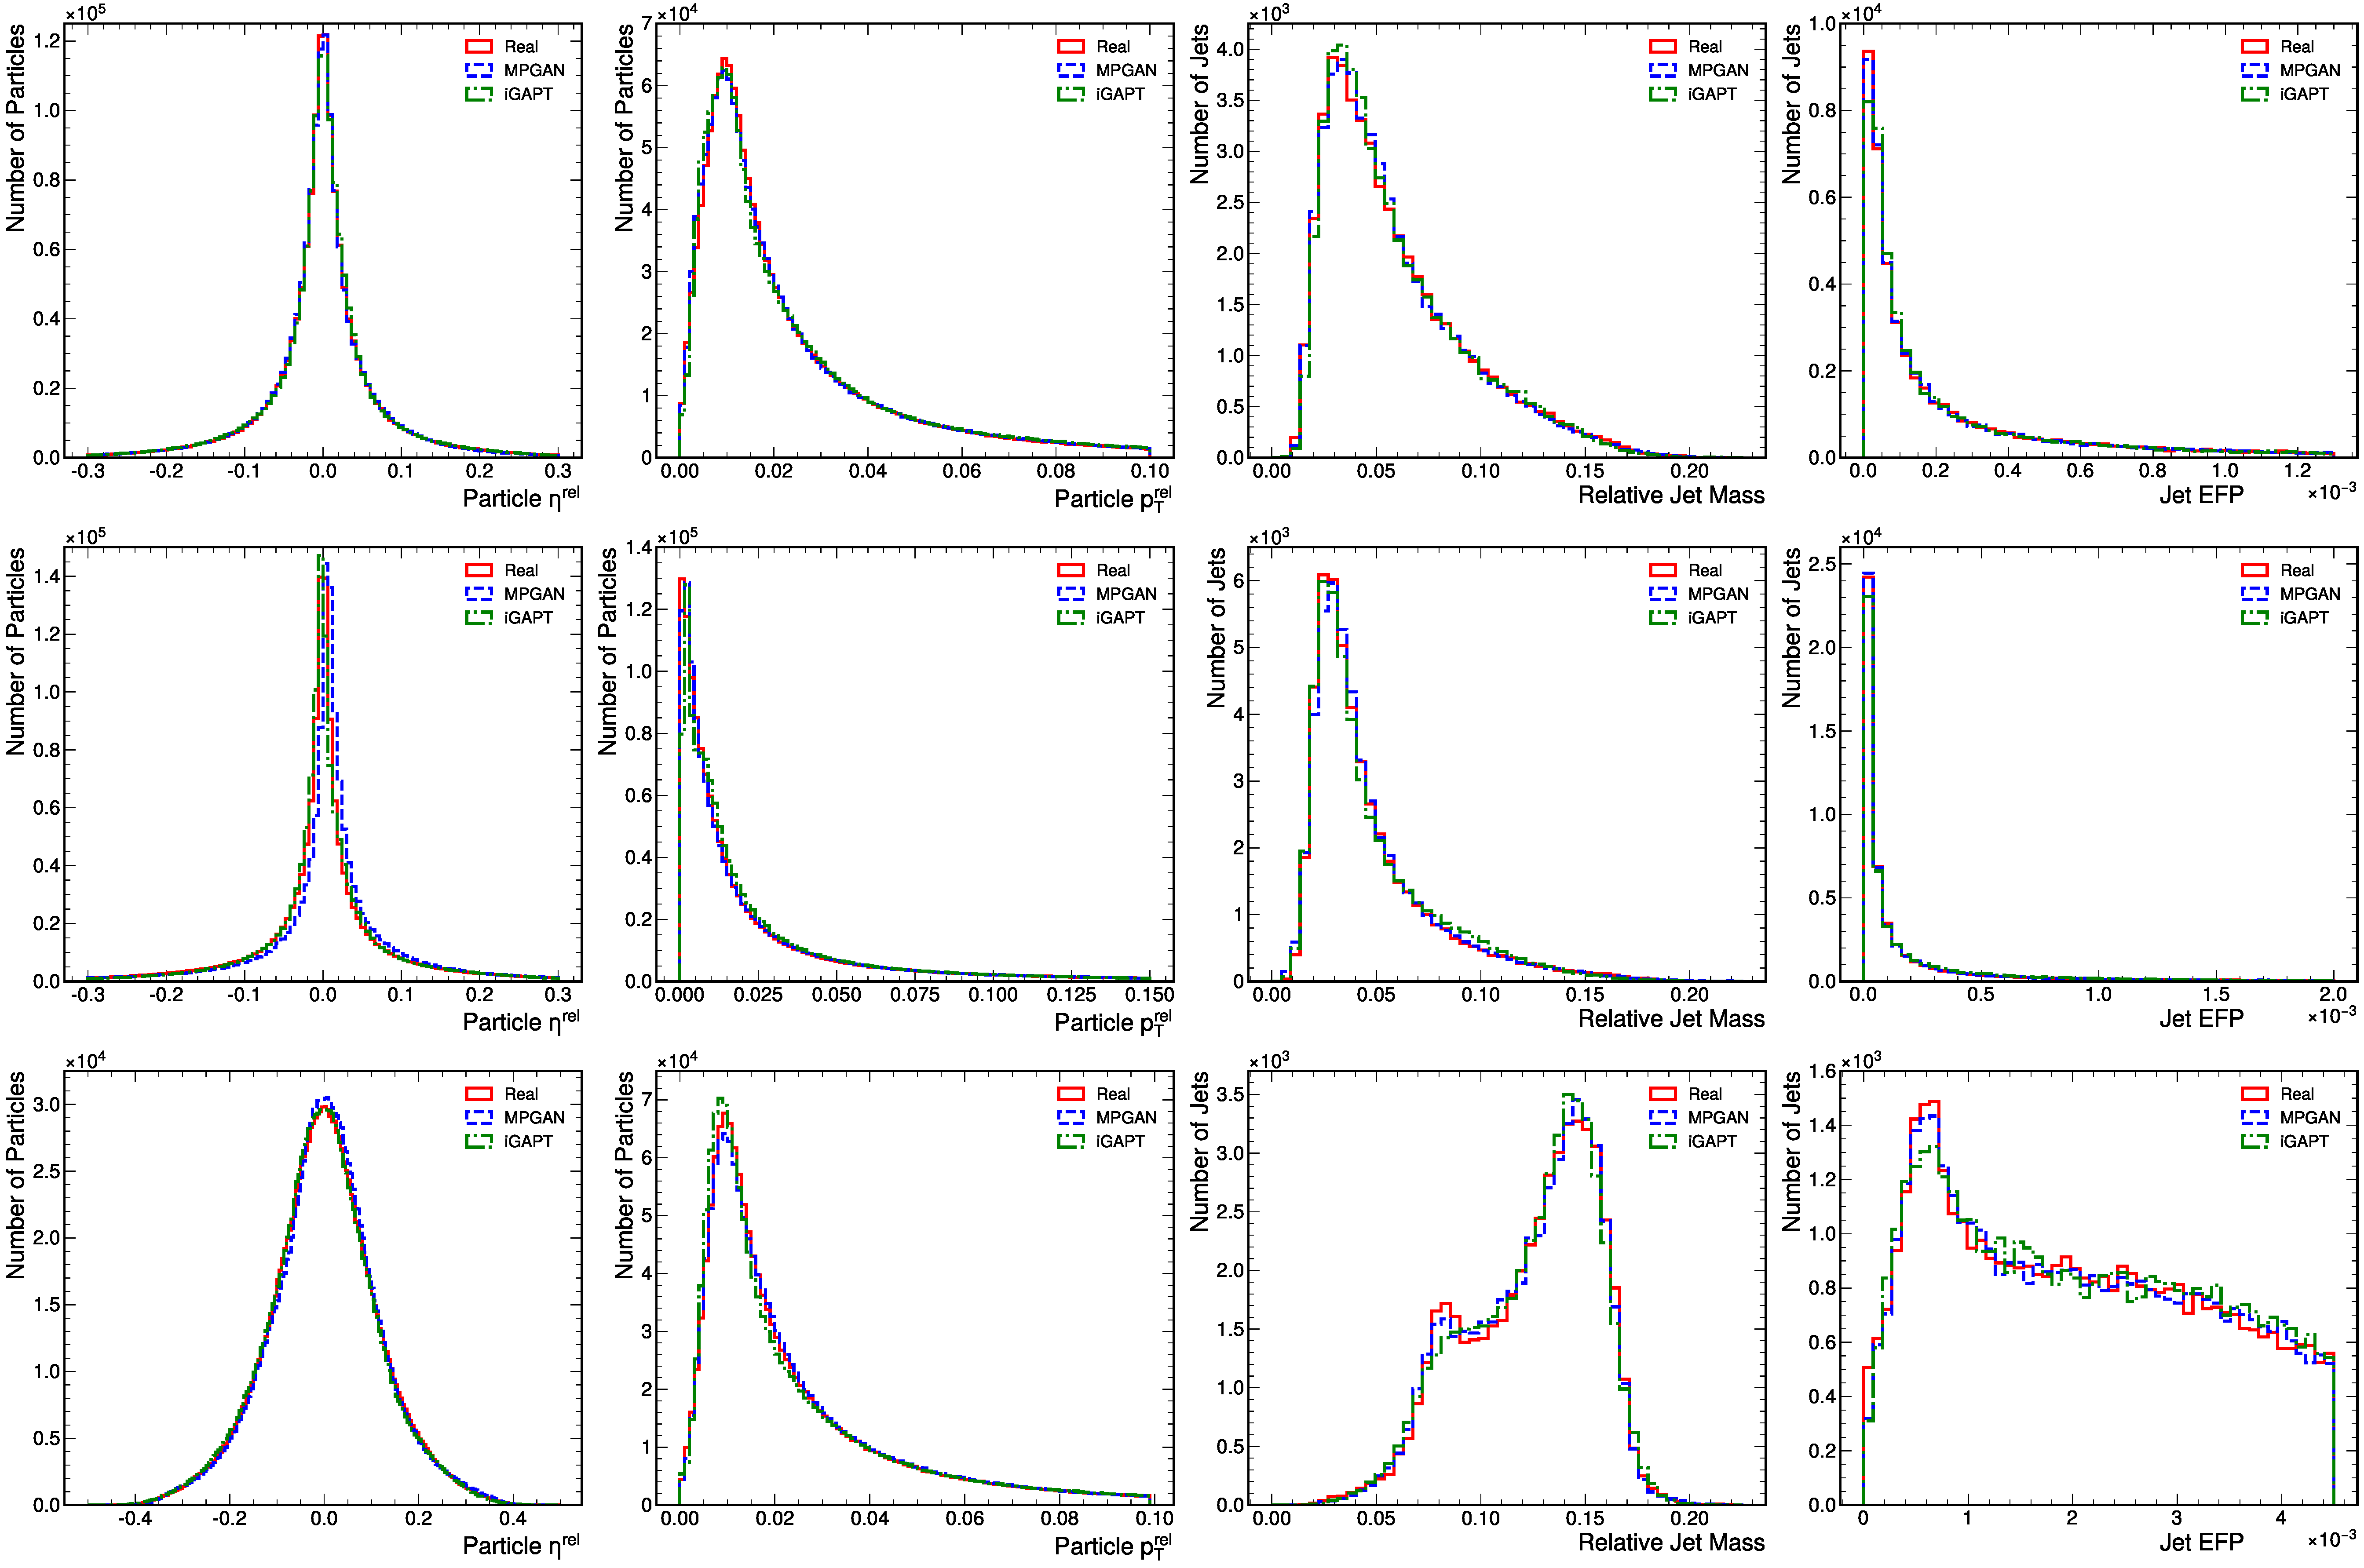
\includegraphics[width=\textwidth]{figures/04-ML4Sim/igapt/feature_distributions_30.pdf}
    \caption[Low-level particle feature distributions (far left and center left) and high-level jet feature distributions (center right and far right).]{Low-level particle feature distributions (far left and center left) and high-level jet feature distributions (center right and far right) for the real data (red), MPGAN-generated data (blue), and iGAPT-generated data (green), for 30-particle gluon (top row), light quark (middle), and top quark jets (bottom).
    A sample $d = 4$ energy flow polynomial~\cite{Komiske:2017aww} is plotted in the rightmost column.
    }
    \label{fig:04_igapt_feature_distributions_30}
\end{figure}

\subsubsection{Timing} 

A key benefit of iGAPT is its improved time complexity over MPGAN.
This is demonstrated in Table~\ref{tab:04_igapt_times_gluon}, which shows the training and generation times for each model for 30 particle jets using the largest batch size possible on an NVIDIA 1080 GPU, with iGAPT outperforming MPGAN by a factor of 3.5.
MPGAN is computationally challenging to extend to 150 particles, hence timing information is not provided; in contrast, iGAPT's training and generation times scale well with the number of particles.
Finally, we note that the ``true'' generation time per jet is approximately 50\,ms (see Section~\ref{sec:04_mpgan_results}), thus iGAPT represents more than a factor of 100 speed up.


\begin{table}[htbp!]
\centering
\caption{Timing measurements for MPGAN and iGAPT, measured on an NVIDIA 1080 GPU.}
\label{tab:04_igapt_times_gluon}
\centering\resizebox{\textwidth}{!}{
\begin{tabular}{l|lccccc}
\toprule
Jet type & Model & Training time & & Generation time & & Batch size \\
 & & (s/epoch) & & (µs / jet) & \\
\midrule
\multirow{2}{*}{Gluon, $n=30$} 
& MPGAN & $193$ & & $142$ & & 512 \\
% & GAPT & 28 & & 1.79 & & 4096 \\
% & GAST & 79 & & 2.64 & & 2048 \\
& iGAPT & \textbf{$31$} & & \textbf{$40$} & & 4096 \\
\midrule
\multirow{1}{*}{Gluon, $n=150$} 
% & MPGAN & - & & - & & - \\
% & GAPT & 92 & & 12.84 & & 512 \\
% & GAST & 229 & & 12.67 & & 512 \\
& iGAPT & $267$ & & $315$ & & 512 \\
\bottomrule
\end{tabular}
}
\end{table}


\subsection{Summary}

We introduced the attention-based generative adversarial particle transformer (GAPT) and induced GAPT (iGAPT) models for fast simulation of particle clouds, and demonstrated their performance visually on the \jetnet dataset.
The iGAPT model, in particular with its induced particle attention blocks (IPABs), offers a significant improvement in time complexity over MPGAN, with promising potential to scale up to the cardinality necessary for (HL-)LHC simulations.

As seen from Figure~\ref{fig:04_igapt_feature_distributions_30}, while visually we can observe roughly that the iGAPT and MPGAN models perform similarly and match the real distributions, this is not sufficient to draw robust and objective conclusions about the models.
In the next chapter, we tackle the problem of quantitatively evaluating and comparing such fast simulators in HEP.

\subsubsection{Acknowledgements}

This chapter is, in part, a reprint of the materials as they appear in the NeurIPS ML4PS Workshop, 2020, R. Kansal; J. Duarte; B. Orzari; T. Tomei; M. Pierini; M. Touranakou; J.-R. Vlimant; and D. Gunopulos. Graph generative adversarial networks for sparse data generation in high energy physics;
NeurIPS, 2021, R. Kansal; J. Duarte; H. Su; B. Orzari; T. Tomei; M. Pierini; M. Touranakou; J.-R. Vlimant; and D. Gunopulos. Particle Cloud Generation with Message Passing Generative Adversarial Networks; and
the NeurIPS ML4PS Workshop, 2024, A. Li; V. Krishnamohan; R. Kansal; J. Duarte; R. Sen; S. Tsan; and Z. Zhang; Induced generative adversarial particle transformers.
The dissertation author was the primary investigator and (co-)author of these papers.